\documentclass[12pt, a4paper]{report}
\usepackage[utf8]{inputenc}
\usepackage{amsmath}
\usepackage{amsfonts}
\usepackage{amssymb}
\usepackage{graphicx}
\usepackage{booktabs}
\usepackage[export]{adjustbox}
\usepackage[style=apa, backend=biber]{biblatex}

%%%%%%%%%%%%%%%%%%%%%%%%% ADD ANY ADDITIONAL PACKAGES BELOW
% Uncomment for blank lines between paragraphs rather than
% indents
\usepackage[parfill]{parskip}
\usepackage{float}

\usepackage{pythonhighlight}

\usepackage[toc,page]{appendix}
\usepackage{pdfpages}

\usepackage{mathtools}
\usepackage{multicol}
\usepackage{mathrsfs}

% testing broken unicode that I can't spot
% \DeclareUnicodeCharacter{200A}{******************************}

%%%%%%%%%%%%%%%%%%%%%%%%%%%%%%%%%%%%%%%%%%%%%%%%%%%%%%%%%%%%

%%%%%%%%%%%%

%  attempt to write wordcount
% Word Count: [1]

% Keywords command
\providecommand{\keywords}[1]
{
  \small
  \textbf{\textit{Keywords---}} #1
}

\addbibresource{refs.bib}

\usepackage[linktocpage=true]{hyperref}	% This creates hyperlinks and moves the contents links to the page number for clarity
% There are lots of options you can alter to what you want, see http://www.tug.org/applications/hyperref/manual.html
\usepackage[font=small,labelfont=bf]{caption}	% This ensures hyperlinks to figures link to the top of the figure not the caption. This line must come after the previous one (hyperref package).
\linespread{1.3}


\begin{document}
\pagenumbering{alph}	% This stops the title page being counted in the page numbering
\thispagestyle{empty}	% This stops a number being put at the bottom
\vspace*{1mm}	% The asterisk is needed because it's at the top of a page

\includegraphics[width=0.85\textwidth, center]{figures/UoP_Primary_Logo_Stacked_pms.eps}
\vspace{8mm}

\begin{center}
% Put the full title  on the front page
\LARGE\textbf{\textsf{Domain analysis of feature implementations between Classic and Deep NLP models.}}\\
\vspace{1mm}
% The student handbook states you need your full name on the front page
\large \textbf{William Green}\\

\vspace{10mm}
\normalsize School of Computing \\ Final Year Project PJE / PJS 40

\vspace{20mm}
%
\today	% This prints todays date, eg. ``January 1, 2012``.
% Make sure all of the above fits on the front page, otherwise you will have to change the spacings, eg. to accomodate a long title
\end{center}
\newpage
\pagenumbering{roman}	% This sets page numbers to be Roman numerals for the preliminaries
\phantomsection	% This makes the abstract's bookmark link to the top of the page instead of the title line.
\addcontentsline{toc}{chapter}{Abstract}	% Gives the Abstract a contents entry
\chapter*{Abstract}	% The asterisk stops a chapter number being assigned

% No more than 300 words summarizing this dissertation.
% APA Abstract Format - 250 words
% Research Problem
% Hypothesis
% Methods
% Results
% Implications

This study investigates the relationship between theory and implementation amalgamations within Natural Language Processing models, researching how the use of older techniques can be brought to life with modern fundamentals for feature extraction of textual classification methods on Student Feedback; this project researched several NLP methods such as Bag-Of-Words, POS-tagging and Word2Vec categorised as Classical, Modern, and Contemporary approaches. To demonstrate the project hypothesis, two indented models were created to display performance differences based on open-source datasets.

This project concluded \ldots This project faced one major limitation, being dataset sample size of student feedback, however, this did not affect the results of the model itself.

Word Count: [8439 --- so far]


\indent \keywords{natural language processing, machine-learning}

\newpage
\renewcommand{\contentsname}{Table of Contents}	% Changes the contents title from 'Contents' to 'Table of Contents' just because it looks better.
\pdfbookmark{Table of Contents}{contents}	% Adds a bookmark 'Table of Contents' in the PDF and labelled 'contents' for the hyperref package.
\tableofcontents

\newpage
\pdfbookmark{List of Tables}{tables}	% Adds a bookmark 'List of Tables' in the PDF and labelled 'tables' for the hyperref package.
\listoftables

\newpage
\pdfbookmark{List of Figures}{figures}	% Adds a bookmark 'List of Figures' in the PDF and labelled 'figures' for the hyperref package.
\listoffigures

% The commands for the preliminary sections below serve the same purposes as for the abstract section above, You can add or remove sections as you see fit.
% Here might also be a good place to put a dedication if you want.
%\newpage
%To...

\newpage

\phantomsection
\addcontentsline{toc}{chapter}{Acknowledgements}
\chapter*{Acknowledgements}
This ones for me.
\newpage


\pagenumbering{arabic}	% Begins normal page numbering for the body of the report.


%%%%%%%%%%%%%%%%% INCLUDE YOUR CHAPTERS BELOW
% If you move the order around, all the cross references remain, sensibly renumbered.
% yay!

% \chapter{Introduction} \label{chap:intro}
A gentle reminder not to get this chapter perfect until the dissertation is nearing its completion\ldots

\section{A section}

\subsection{A sub-section}

\subsubsection{A sub-sub-section}



\section{Citations}

When it comes to referencing, if we want to assert a fact and then provide its reference use \verb!\parencite!. For example -- one should adapt feedback to learner personality \parencite{dennis2016adapting}.

Or if you want to talk about the research directly, use \verb!\textcite!: \textcite{dennis2016adapting} did a PhD in adapting feedback to learner personality. 

If you want to cite two sources at the same time, you can separate the keys with commas \parencite{dennis2016adapting,cle12}.

\section{Figures}

\begin{figure}
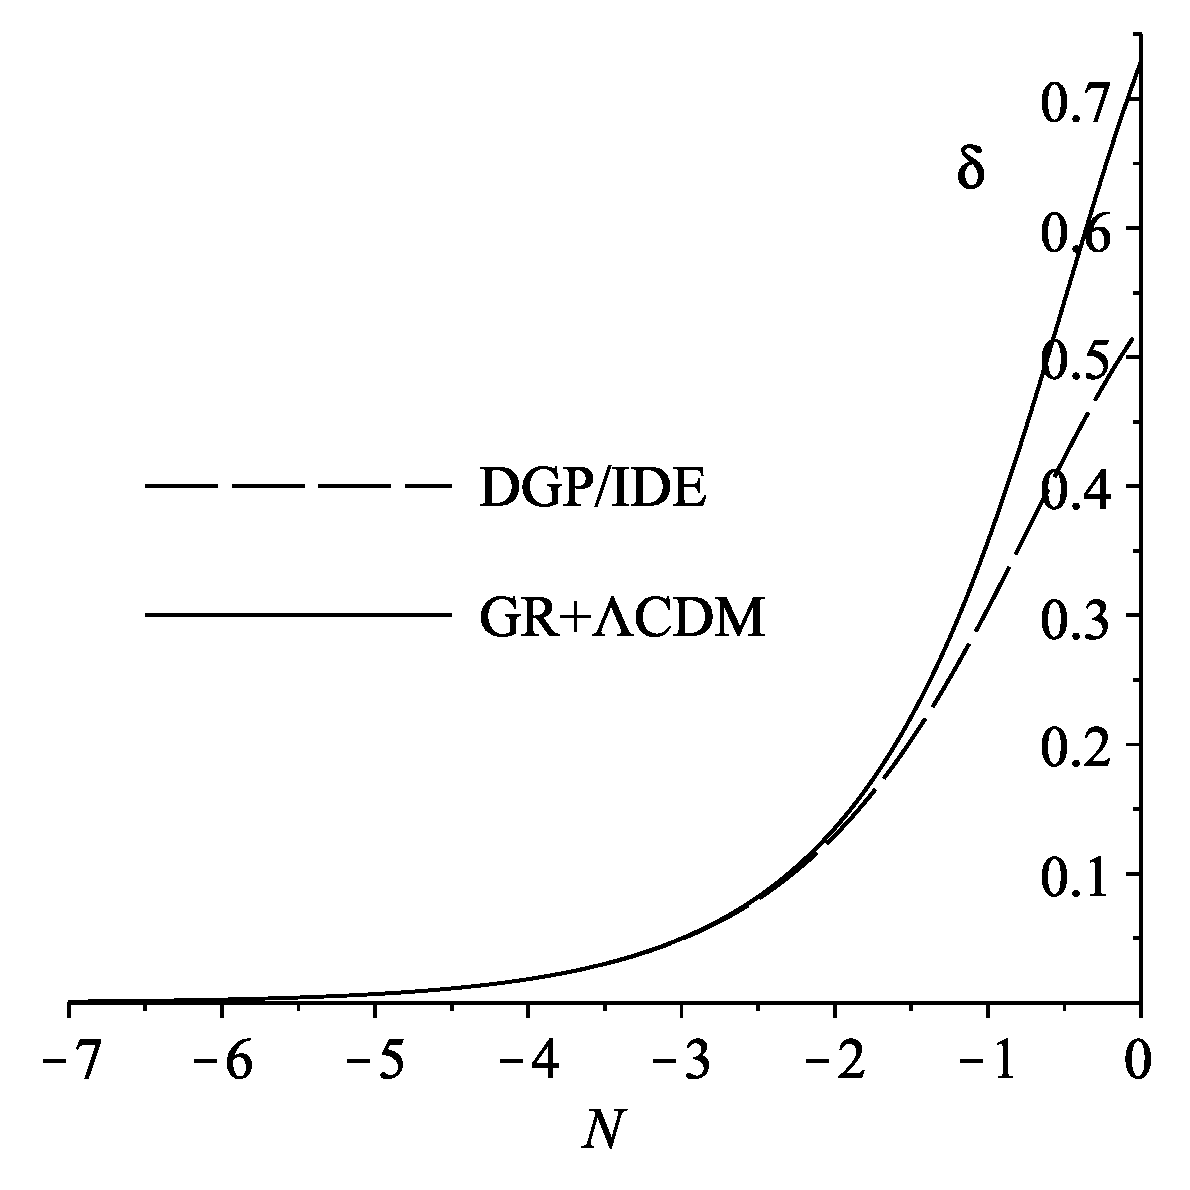
\includegraphics[width=0.49\columnwidth]{figures/dgpdeltas.eps}
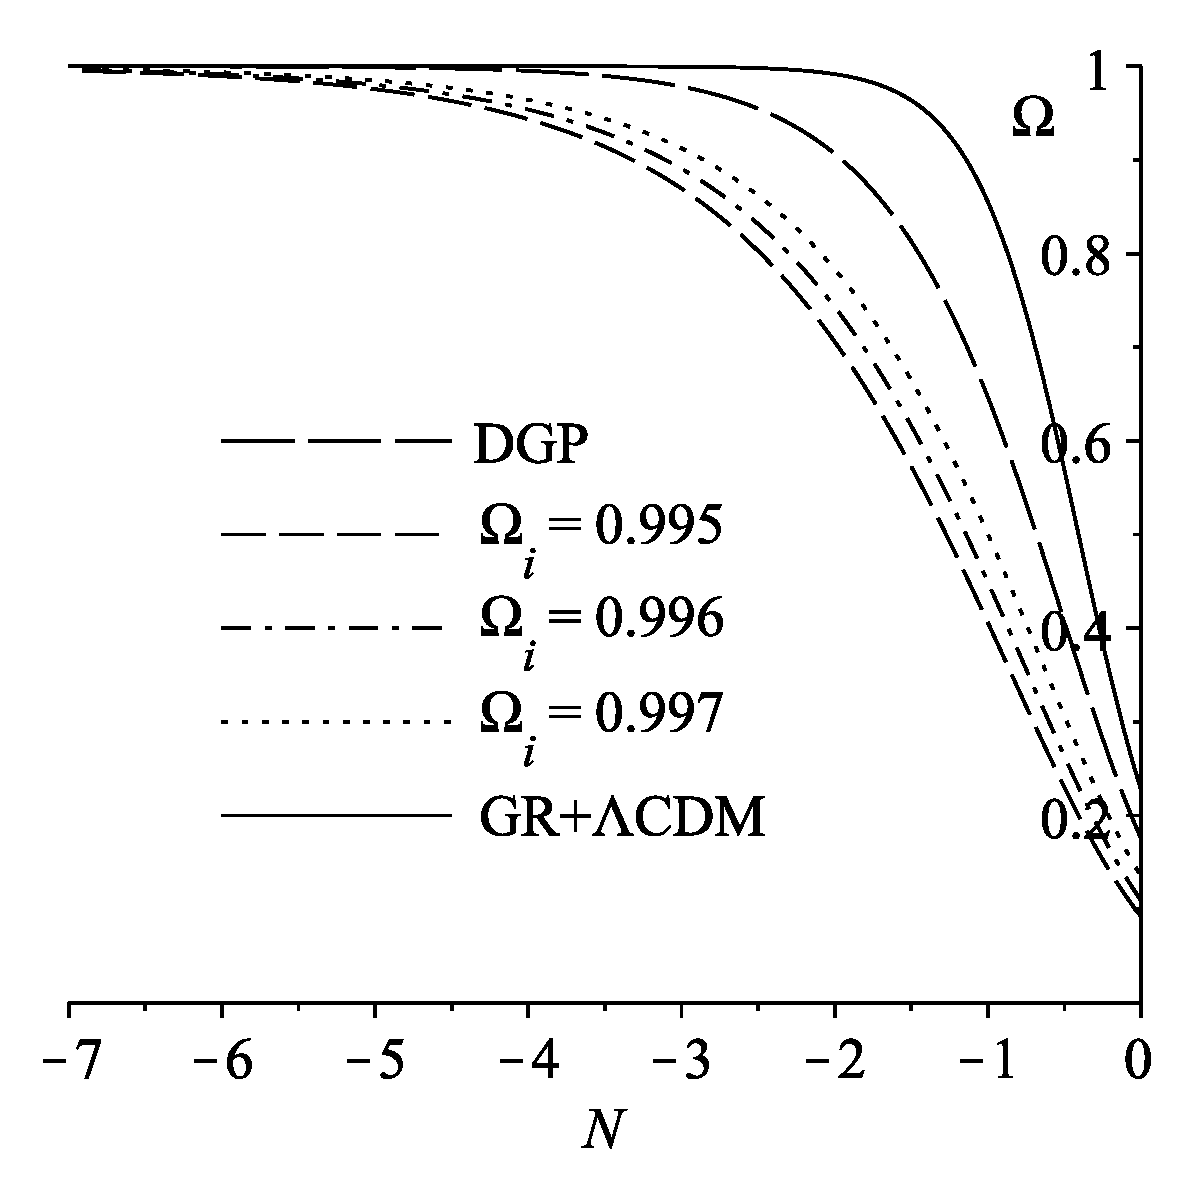
\includegraphics[width=0.49\columnwidth]{figures/dgpomegas.eps}
% For long captions include a short version for the List of Figures/Tables sections in square brackets as below.
\caption[Evolutions of $\delta$ and $\Omega$ for DGP]{Evolution of the density perturbation (left) and the density parameters (right) for the matched DGP/IDE models, each with a different $\Omega_i$,
and a GR+$\Lambda$CDM model.
\label{fig:matched}}
\end{figure}

Don't the graphs in \autoref{fig:matched} look scary? Don't worry, this is because I adapted this template from ICJS. Remember - if you are including screenshots or other raster graphics (i.e. PNG, JPEG) you should ensure that they are at least 300dpi. This will take effort on your part - most people's screens are at 72dpi.   

Vector is better (EPS or PDF) if you can manage it. If you are exporting graphs from Microsoft Excel for example, place the chart in its own sheet and print it to PDF. Then, using Acrobat or similar, crop the whitespace off the PDF. This is the most reliable way I have found to include vector graphics from Microsoft Office.







% To include math symbols in things with hyperlinks you need to specify an alternative plain text version for the bookmark using \texorpdfstring as below:
\section{A section with math symbols, eg. \texorpdfstring{$\Lambda$}{Lambda}CDM}
test test test test test test test test test test test test test test test test test test test test test test test test test test test test test test test test test test test test test test test test
test test test test test test test test test test test test test test test test test test test test test test test test test test test test test test test test test test test test test test test test
test test test test test test test test test test test test test test test test test test test test test test test test test test test test test test test test test test test test test test test test
test test test test test test test test test test test test test test test test test test test test test test test test test test test test test test test test test test test test test test test test


% 
\chapter{More examples}

\section{Equations}

Here's an equation,
\begin{equation}
E=mc^2.\label{eq:einstein}
\end{equation}

\noindent I can reference that easily in the text: \autoref{eq:einstein}. It's even a hyperlink. How nice. 

\section{Opening and closing quotes}

Unlike modern word processors, you need to specify in \LaTeX{} which quote mark to print. To get an opening quote you use a backtick and the regular apostrophe for a closing quote. Double them up for speech. ``This isn't so hard after all''. One just needs to `get used' to it. 

One should never use an apostrophe for plurals. Nope, not even for abbreviations, e.g. in the 1990s, people bought CDs from Virgin Megastores. 

In the \textbf{extremely} rare cases where it's unclear, match it with an opening quote if you must. I got three `A's for my AS Levels. 

\section{Tables}

Tables are joyous fun. The \verb+tabular+ environment is the most common, although it's rather old fashioned and wrangling it into doing what you want can be arcane. Happily, tablesgenerator.com can produce tables from a visual editor or paste from word.

A few things to help you unlearn bad table habits:

\begin{itemize}
    \item You should not use vertical lines in tables. Seriously -- this is an awful 1990s era default from Microsoft Word which has hung around and never gone away. 
    \item the booktabs package can make prettier tables (vertical lines are intentionally banned) - select this option in tablesgenerator. I have included the package for you
    \item You should use tables for comparing numerical data and not as a way of laying out content or paragraph text
\end{itemize}

\begin{table}
    \centering
    \begin{tabular}{lccc}
        \toprule
        \textbf{Feature} & \textbf{Liked (\%)} & \textbf{Disliked (\%)} & \textbf{Didn't know (\%)}  \\ \midrule
        Vertical lines & 0 & 90 & 10 \\
        Using Word & 40 & 40 & 20 \\
        \bottomrule
    \end{tabular}
    \caption{Made up percentages of participants that liked random features}
    \label{tab:sample}
\end{table}

\noindent \autoref{tab:sample} shows a simple table made by hand by yours truly. Note that the column separator is \& which means you must always escape that character if you want to use it in text.





\chapter{Introduction} \label{chapter:Introduction}

This report focuses on the theoretical differences of how Natural Language Processing (NLP) models are implemented and subsequently how performance is affected with certain technical abilities, a key aspect of this report will demonstrate the question “does adding new to old bring enhancements?”. This chapter will cover the technical context of this project and report, the aims, objectives and introduce the domain in which this project lies. Natural language processing is subtopic topic covering and interconnecting computational theory, artificial intelligence/ machine learning and linguistics.

To consolidate the theoretical findings throughout technical chapters, this report will include two variants of a traditional NLP model that represents how a specific NLP technique is implemented. The aims of this project are to produce two machine learning models in which outline if and how traditional NLP techniques can be enhanced using modern theoretically driven techniques; the fundamental ideology of this project is to explore amalgamating NLP concepts and techniques to seek performance increases for dataset dependant models, the specific domain for this project is NLP in academia with the dataset being focused on Student Feedback Surveys. As seen in Chapter 2, we can expand our specific intention for this project and dataset to produce a novel NLP model on how to predict Student Feedback using the same techniques.

\section{Background and Context}

Natural Language Processing has been relatively overlooked during the boom of machine learning, its fundamentals have not changed as there has not been a reason to progress at the same rate as other areas in “Artificial Intelligence”, by adapting well---known theory, it is possible to progress the computational abilities of NLP. The background of this project is to bring modern approaches to older implementations with the justifications being student feedback surveys as the domain.

This project will be looking at areas from: Text and Speech Processing, Morphological Analysis, Syntactic Analysis and Lexical Semantics to give breakdowns of how they could function together to provide a potentially more efficient model.

\section{Project Aims and Objectives}

To successfully validate my project statement, there are several underlying implications that project aims must establish; the aims of this report are to compare the theory behind classical models and machine learning models of NLP and its subcategories of linguistics, such as grammar and text classification. This report will be corroborated using programming artifacts shown throughout, they will feature two NLP models, one of which demonstrates classical implementations on a given dataset and the other demonstrates an adapted form of a classical implementation with additional ML theory and techniques.

These aims will be achieved by meeting the following objectives:

\begin{itemize}
    \item Contrasting and comparing types of NLP techniques in a specific domain
    \item Research and provide results for adding ML techniques to a traditional method
	\item Compare older methods to modern methods
	\item Speed advantages or disadvantages when combining different methods and implementations
	\item Using research from this disco comparing POS tagging and word2vec with ML implementations for text classification and sentiment analysis using the results
\end{itemize}

By meeting these objectives, this project will have highlighted a novel approach expored in \autoref{chapter:ProjectDesign} to text classification and minimising computational costs whilst having no detrimental effects to accuracy.

\section{Deliverable}

Project Deliverable: compilable Python object.

\section{Project Constraints and Risks}

The biggest constraint for such a problem---related project is one of time, including time management; the approach of this project is to reflect on current theory to understand how to implement a novel solution to a specific application’s domain, as implementations of Text---Classification are heavily theory dependant where each topic has a broad overview, it seems time will be of essence. A secondary constraint to this project may be inherited from a programmatic approach, whereby language features, libraries, or framework versions may have conflict.

\section{Risk Assessment and Mitigation}

This project's risks can be categorised as three major areas:

\begin{itemize}
	\item \textbf{\textit{Developer illness:}} Impact on project is subjective to the degree of severity.
	\item \textbf{\textit{Delays in communication:}} Due to COVID-19 and on-going pandemic, specifically "working from home".
	\item \textbf{\textit{Inadequate training data/ sample size:}} As a machine-learning based project, ample data is needed for successful training.
\end{itemize}

As seen in \autoref{appendix:AppendixPID}, there is a table outlining the risks and negative impact factors associated with this project from its initialization; this table is included for risks in \autoref{chapter:Introduction} as they have already been signed off and approved.

\begin{figure}[H]
    \centering
    \includegraphics[width=\textwidth]{figures/chapter-1/PID-Risk-Table.png}
    \caption[PID-Risk-Table]{PID-Risk-Table.
    \label{fig:PID-Risk-Table}}
\end{figure}
\chapter{Literature Review}

The focus of this chapter is to analyse and breakdown current research and literature concerning the use of NLP models within a domain and their implementations, specifically looking into the area of academia. The domain for this research will be text classification on Student Feedback forms; NLP has many interconnecting domains, in which implementations can heavily affect performance and the returned results. As the theory behind NLP grows, it is vital to use the least computationally cost---effective methods in which this section will be looking at merging newer techniques with older models to potentially improve our understanding of NLP models.

\section{What is NLP?}

Fundamentally, Natural Language Processing is an area of Computer Science which enables computer systems to access and understand human linguistics \parencite{eisenstein2019introduction}, expanding, NLP is theoretically driven computation for the purpose of evaluating, interpreting, and depicting naturally occurring transcripts to a certain level of detail. Differing depths of linguistics are used for analysis in---order to return a desired human---like range of processing for a particular application (needs the cite).

Over the last 20 years, NLP has become an integral topic of Computer Science as it combines computational linguistics with a popular buzzword Artificial Intelligence or more accurately Machine Learning \parencite{ongsulee2017artificial}, these terms have been generalized as this area of computing heavily relies on theory from different departments. Human and machine communication mediums both have similarities, to which we can model our understandings on, syntax is an intrinsic value to both communications, and it is used to label every component of a language and its sets of rules \parencite{jain2018natural}.

The value of NLP is in its ability to remove ambiguity in linguistic forms, this explicitness results in a clear data---driven numeric structure for numerous types of applications \parencite{SAS2021NLP}. The returned data structures are a result of some form of input, NLP algorithms can handle speech, text, or images where of the appropriate architecture. The properties and potentials of NLP are now used for commercial spaces and for public interest, several areas including:

\begin{itemize}
    \item Machine Translation
    \item Speech Functions
    \item Dialog Interfaces
    \item Text Analysis
    \item Natural Language Generation
    \item Writing Assistance
\end{itemize}

The list above outlines six key areas of NLP that are used in commercial spaces and the majority appeals to the academic space; the listed six areas are a high---level overview at how different theoretical approaches combine in---order to perform a given task \parencite{dale2019nlp} for the purpose of this literature review, we will be looking at the most relevant areas in which aid this domain.

\section{Uses of NLP in Academic Institutions}

As NLP expands, so do its domains; a more recent use of NLP is within academic institutions. During the last term of a module, it is common for universities to collect data regarding its practices and teaching etiquette. Universities will utilize both formal and informal techniques for elicitation, typically a printed hand---copy or via an online questionnaire, thereafter student feedback is analysed to provide institutions with a gauge on how to improve students’ satisfaction, module content, structure, and teaching methods. Information elicitation is completed in the form of a survey, with two main question approaches, being “program---wide” and “module---specific” to target flexibility of opinion vs factual coverage \parencite{keane2005obtaining, beran2007s}.

During the academic year of 2019/2020, education became distanced due to COVID---19 and accordingly E---learning soared as academic institutes were forced to adapt their teaching mediums and operations to become temporality online only \parencite{burgess2020schools}, this resulted in a frequent uptake of online feedback. This surge of sudden online academia has resulted in rapid development of Massive Open Online Courses (MOOC), these E---learning platforms enable student feedback on an extensive scale with reputable data to develop and train NLP models \parencite{wang2021predicting}.

The data gathered is used to give insight if users are satisfied with their academic consumption, NLP methods can be applied to student feedback to give the academic institution an idea if its students are validating the unified theory of acceptance and use of technology (UTAUT) model \parencite{kayali2020adoption}. Large data sets such as a class of 200 students would be tedious and time consuming for a lecturer to manually analyse individual feedback; combining aspects of staff roles and deep learning would utilize the computational power required for sizeable datasets by minimizing the required engineering \parencite{lecun2015deep}.

Manual thematic analysis of a dataset to formulate codes and themes also allows for human error, poor judgement as interpretation is subjective, and themes may be overlooked \parencite{belotto2018data}. As more aspects of data---driven interactions between clientele can be applied to NLP, the development of an all---purpose, accurate and, secure method to automating the elicitation of necessary linguistic aspects from an input source is increasingly imperative \parencite{sindhu2019aspect}.

A generalised approach for analysing student feedback is with the use of Word Embedding, popular implementations are Word2Vec, GloVe \parencite{pennington2014glove}, and FastText \parencite{edalati2020potential}.

\section{Applicable Methods for Text Classification on Student Feedback}

The intended outcome is to evaluate student feedback surveys which will be targeted towards enhancing the level of learning and engagement by students; to achieve the desired results, the following techniques would be most suitable if appropriately applied in this context.

\subsection{Sentiment Analysis and Opinion Mining}

The desired outcome is to derive subjective material from students’ input, this can be insights, discussions or opinions which automatically review the polarity (negative, neutral, or positive) of information regarding the academic facilities \parencite{kandhro2019student}. Sentiment Analysis has three levels of scope which can be reduced to emulate different levels of comprehension:

\begin{figure}[H]
    \centering
    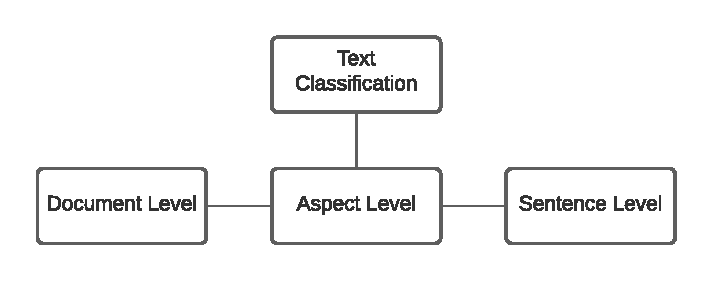
\includegraphics[width=\textwidth]{figures/chapter-2/TextClassificationTaxonomy.pdf}
    \caption[Taxonomical overview of Text Classification Levels]{Taxonomical overview of Text Classification Levels}
\end{figure}

\newpage

\textcite{kastrati2020weakly}, established an aspect---orientated opinion---mining model; student feedback was in English (Natural Language)  whereby three unique NLP techniques were applied to the dataset to produce three represented perceptions of the same dataset. The NLP techniques applied were: Word Embedding, Term Frequency (TF) and Term Frequency---Inverse Document Frequency (TF---IDF).

\textcite{kastrati2020weakly}, trained their models using already explored classifiers, Decision Tree, Naïve Bayes, Support Vector Machines and Boosted Graphs on a 1---Directional Convolutional Neural Network (1D---CNN). \textcite{kastrati2020weakly}, found traditional aspects of Machine Learning implementations yielded greater results than that of the sole use of a 1D---CNN.

\textcite{kastrati2020aspect} “Aspect---Based Opinion Mining of Students' Reviews” (2020) to produce a weakly supervised framework aimed at training deep learning models with little to no human interaction. Their proposed framework analyses a desired sentiment at document level and yielded an overall F1 score of 86.13\%  accuracy; they also tested their framework at the aspect level for sentiment analysis to which yielded an F1 score of 82.1\%. The logic of this paper is applicable to this project as the framework is appropriate as little human involvement will occur when training and saw a similar F1 scoring.

\subsection{Topic Labelling}

This technique is used in conjunction with text mining to automatically handle significant and reoccurring themes and topics within students’ feedback with automatic creation of category labels per survey and section. Latent Dirichlet Allocation (LDA) is a suitable model which can achieve the above, it uses Latent Dirichlet Distributions to group topics as a multinomial distribution of words and is able to associate words based on the probability distribution of the set \parencite{unankard2019topic}.

\subsection{Language Detection}

This technique of NLP deals with determining which natural language (NL) is provided as the input source, this approach could be particularly beneficial to lecturers if the student and lecturer do not share the same first language; a classifier could be challenged by identifying an incorrect NL due to lexical and syntactical resemblance. These challenges could return pedagogical ambiguities within feedback \parencite{heift2017computer}, if a lecturer misinterprets student feedback due to a misunderstood lexical, an unintended impression will be represented.

This can be aided by converting NL structures in to a first---order logic (FOL) object to which these mathematical models will return the highest matching lexical in a percentage \parencite{perikos2017assistance}. Therefore, minimising miscommunication.

\subsection{Intent Detection}

This technique is used to programmatically classify implied intent within an input, based on a certain ambition or outcome, usually a verbal adjective. Every student feedback survey has the same interaction purpose, to improve their quality of learning, this specific domain can be modelled to automatically categorise each intentional improvement specification. Intent classification can also be used to provide real---time feedback to lecturers opposed to standardised question---answer dialog systems \parencite{jensen2020toward}.

A common implementation of intent detection is with the use of a rule---based model, these systems use predefined constraints as intents with the hypothesis that occurring utterances conform with the predefined set of rules. These rules will be disputed when a novel utterance is parsed, as students have different methods of expressing their views, novel utterances will be frequent and with the appearance of utterances without a predefined label will increase, this problem exists under Zero---shot learning with CNNs \parencite{xia2018zero}.

However, textual classification is still an area of development and is not well---understood with regards to the most appropriate implementation, algorithm, and paradigm combination \parencite{thangaraj2018text}. An inherent objective of this paper will be looking at the amalgamations of theory to return the most effective and efficient results driven implementation for domain specific feedback classification.

\section{Related Research}

This section will predominantly concentrate on considerable studies of similar nature and existing solutions such as open-sourse libraries, the focused studies conduct research spotlighting technical performance of differing textual and contextual classification methods using different datasets and NLP models.

\subsection{Related Systems and Libraries}
% TODO insert table with huggingface spacy etc...

\begin{table}[H]
    \centering
    \begin{tabular}{|c c c c|}
        \hline
        Software Title & Type & Pros & Cons \\ [0.5ex]
        \hline
        Bert & Library & Everything & Nothing \\
        \hline
        Hugging Face & Library & Everything & Nothing \\
        \hline
        SpaCy & Library & Everything & Nothing \\ [1ex]
        \hline
    \end{tabular}
   \caption{Aggregation of current available software systems and libraries.}
   \label{tab:C2RelatedSystems}
\end{table}

Analysing previous literature will guide further development as they will give support towards vital features that are a prerequisite for essential system requirements, to the contrary, previous literature may outline features that are not of importance and potentially expose gaps in current research.

\subsection{Combination Classifiers}

The completed work in “a comparative study of classifier combination applied to NLP tasks” by \textcite{enriquez2013comparative}, was viewed as a comprehensive comparison and overview of diverging NLP implementations and combining methods for exercised NLP workloads. Enriquez and colleagues’ findings suggested lesser explored NLP models and classifiers yielded higher performance opposed to well---known implementations, for example, the combination of “stacking” anchors and “cascading” input layers for Part---of---Speech tagging returned results exceeding expectations \parencite{enriquez2013comparative}.

The fundamental concepts \textcite{enriquez2013comparative} encountered are applicable to modern development of combination classifiers; when developing a novel combination model, there are two compulsory criteria that must be met to be successful: heterogeneity of the chosen classifiers, this ensures a computational mistake will only be met once and will be provided a differing perception to an encountered error; veracity of the chosen classifiers, each classifier must reduce the occurrence of inaccuracies over another selected classifier.

An additional audit should be performed to verify the certainty of the desired classifiers will work together: statistical, are the chosen classifiers best suited? Given the problem based on previous resources; computational, accounting for time and space complexity, is there a potential to reach computational limits? That affect the desired result; representational, has the classifier been previously research to understand the objective task? Considering the criteria above, \textcite{enriquez2013comparative} chose to investigate:

\begin{itemize}
    \item Voting
    \item Bayesian Merging
    \item Behaviour Knowledge Space
    \item Bagging
    \item Stacking
    \item Feature Sub---spacing
    \item Cascading
\end{itemize}

The above NLP methods and techniques were applied to 9 different corpuses to train models for Part---of---Speech Tagging.

Since the work of \textcite{enriquez2013comparative}, NLP methods have advanced, more up---to---date findings reviewed in the paper “Prediction of Sentiment Analysis on Educational Data based on Deep Learning Approach” by \parencite{sultana2018prediction} centralises eight classifiers for performance inspection in which they are put against each other for speed, accuracy, and computational cost. This paper includes an open---sourced educational dataset from Kiteboard 360 which is provided to the individual classifiers, the classifiers tested were:

\begin{itemize}
    \item Support---Vector Machine (SVM)
    \item Multi---layer Perception (MLP)
    \item Decision Tree
    \item K---star (K*)
    \item Bayes Net
    \item Simple Logistics
    \item Multi---Class
    \item Random Forest
\end{itemize}

The dataset was parsed to each classifier to create a trained model, the results were then investigated and corroborated with dummy data; if the returned object was valid, it was evaluated by metrics. Scoring against metric such as returned accuracy, RMSE, specificity, sensitivity, F1 percentage and Receiver Operating Characteristics (ROC) curve area to compare performance to conclude the most valuable model for a given dataset \parencite{sultana2018prediction}. According to Sultana and colleagues, SVM and MLP implementations are perceived as the two surpassing models in comparison for applying NLP techniques to student feedback.

\subsection{Constructing a New Combination Classifier}

When attempting to create a novel approach to a widely researched area, challenges will be faced due to the theoretical capacity of current implementations; coverage on current methods must be known to be able include adaptions for a successful improvement. The review work of “Text Classification Algorithms: A Survey” by \parencite{kowsari2019text} provides in---depth insight for the construction and expansion of already implemented algorithms.

\textcite{kowsari2019text} summarised the construction of text classification algorithms in real---world applications share four key aspects, in which can be dismantled into “feature extraction”, “dimension reductions”, classifier selection”, and “evaluations”; phase 3 of \textcite{kowsari2019text} process is complemented by \textcite{enriquez2013comparative} findings on how to choose an appropriate classifier.

\textcite{kowsari2019text} first addressed that the scope of the classifier must be identified, according to the scope levels of Sentiment Analysis in Figure 1. Phase 1 being feature extraction handles the source input, namely unstructured datasets that must be converted to an acceptable object for a classification model, this includes cleaning and formatting of the object.

Phase 2 being dimensionality reduction will handle the acceptable object to check for high costing computational executions, this allows a classification model to make use of low costing functions without decreasing accuracy, it also allows for pre---processing to take place rather than using inexpensive classification models; the aim of phase 2 is reduce the time and space complexity of a classification method.

\textcite{raunak2019effective} proposed a novel approach on how to handle datasets where dimensionality is a computational issue, Raunak demonstrated the use of pre---trained word embedding models for all depths of a document with emphasis on reduced space complexity. The proposed model uses the combination of the Parasitism---Predation Algorithm with Principal Component Analysis as a post---processing layer to filter irrelevant lexicons.

Phase 3 is simply identifying the most appropriate classification pipeline. Phase 4 is evaluation, there are many ways to evaluate how a classification model performs but the most important are speed and accuracy \textcite{kowsari2019text}.

\subsection{Identifying Research Gaps and Including Novelty} \label{section:IdentifyingResearchGapsandIncludingNovelty}

The purpose of reviewing existing literature is to understand how current research and findings are being used to expand a topic’s theory; the aim of this section is to compile accepted theories, identify common themes from background knowledge, and to distinguish potential gaps in existing literature to provoke the creation of a novel NLP idea and methodological schematic.

This section identifies two suggestions based on concurrent themes in this report; one is suggestive to the theoretical workings of this paper and the other is suggestive to domain specific feature applications.

Many comparative studies overlook how the interaction between simplistic aspects of traditional approaches can be benefitted by incorporating machine learning aspects such as (Convolutional or Recurrent) Neural Networks can affect classification performance. As NLP grows, the comparison between POS---Tagging and evolved versions of Word2Vec have also been overlooked, studies such as “Recent Trends in Deep Learning Based Natural Language” by \parencite{young2018recent} directly compare linear implementations of statistical analysis but do not look at non---linear Word2Vec advances such as SPvec \parencite{zhang2020spvec}, this will be expanded on in section \ref{section:DerivedfromLiteratureReview}.

\textcite{suleiman2019using} state that Word2Vec is an efficient model for word embedding, however think it can be improved with an extension, their proposed model explores how POS---Tagging could enhance the probabilistic values of results returned by Word2Vec models as POS---Tagging calculates a higher vector between feature semantics. Whilst covering Word2Vec implementations with POS---Tagging, they did not cover fundamental analysis of how POS---Tagging effects Word2Vec’s facets such as POS---Tagging with CBOW vs Skip gram algorithms; item 1’s “enhancement” could refer to the use of character n---grams to ensure the importance of Word2Vec word---order. this will be expanded on in section \ref{section:DerivedfromLiteratureReview}.

According to Sultana et al., (2018) applied SVMs yielded greater results when combined with a textual classification technique and was the building block for item two; the justified domain being student feedback can be promoted to predicting student feedback based on existing results and Text Frequency Analysis \parencite{alqurashi2019predicting}.

\textcite{alqurashi2019predicting} proposed a new framework with four key factors to measure student satisfaction; 167 students completed a designed survey targeted at course interaction and perceived learning. Using a 5---point score system, the results indicated that student learning interaction had little effect on the prediction model, with score of 0.1\%. Alqurashi’s findings are important as it gives insight to which labels should be parsed based on importance to train a new predication model for topic labelling, suggested in section 2.3 which in turn validates the findings of \parencite{unankard2019topic} for topic detection.

\chapter{Methodology and Project Management}

When managing the development of a project, there are several approaches one can take when planning the development lifecycle \parencite{shylesh2017study}; the three main approaches for any project are sequential (linear), incremental, and iterative (non-linear) phases \parencite{akinsola2020comparative}, which methodology is best suited depends on the nature of the application. The nature of this project involved one developer with evolving requirements, adaptable features, and unforeseen management issues, therefore the following methodologies were explored and appropriately chosen.

The planning and development carried throughout this project were based on an agile methodology model designed for specific and individual use. This section discusses how to differentiate between the most appropriate and applicable methodology, to which will establish the final selected software development lifecycle model (SDLC). The scope for this project can be displayed as such:

\begin{figure}[H]
    \centering
    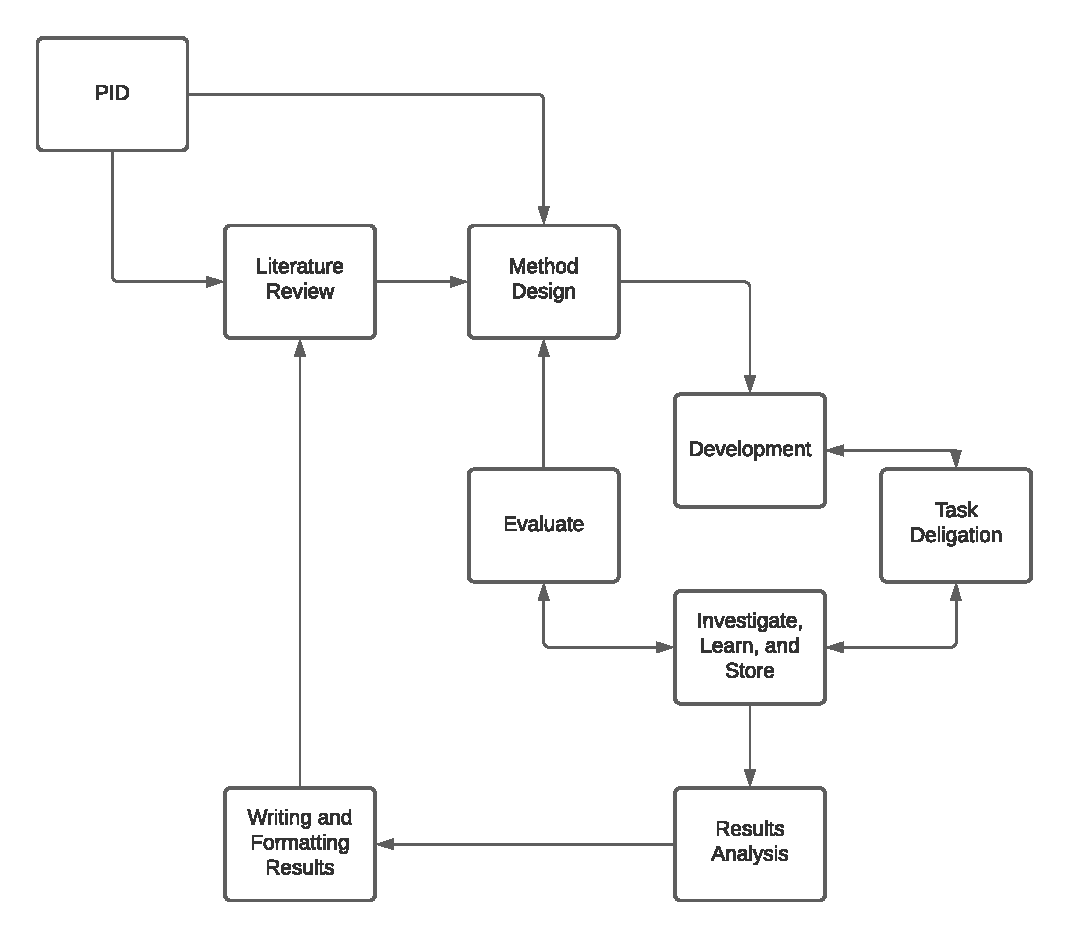
\includegraphics[width=\textwidth]{figures/chapter-3/ProjectOverviewFlowChart.pdf}
    \caption[Overview of Project Workflow]{Overview of the project from start to finish
    \label{fig:ProjectWorkflow}}
\end{figure}

As seen in \autoref{fig:ProjectWorkflow}, this project follows an iterative process with included circular motion for data validation and section corroboration. Due to this nature, it seems a hybrid SDLC Model is best suited for this project; the apparent combination of methodologies allows for aspects from both strict Test-Driven Development and Rapid Application Development without the inclusion of their inherent disadvantages.

Whilst the original commencement plan for this project was entirely constructed on the Waterfall Model as depicted in the supplied Gantt Chart within the PID document, this however, was not a sufficient process mainly due to time constraints, thus the Waterfall Model structure was partly ignored to allow for improved efficiency requirements and minor tweaks to previously stated tasks. These tweaks are outlined in the final chosen (adapted) model.

\section{Methodologies}

This project uses two SDLC’s, one for the project in its entirety and one for development.

\subsection{Data Mining}

This project’s primary objective is text classification which focuses on predictive aspects of NLP, data mining and analytics are inherently used in machine-learning and natural language processing as for a model to be predictive there must be a history of data to be analysed, this project uses openly sourced student feedback from Kaggle to achieve clean and rich data without breaching ethical concerns.

Big datasets are becoming widely used for research and data-mining techniques aid development as they ensure the correct dataset is being used, appropriate data must be used for the applied techniques and data manipulation because inappropriate data could lead to inaccurate or misleading results. It is essential that the use of data is appropriate for the proposed machine learning model, in the scope of this project it is student feedback being mined and analysed through a predictive model.

\subsection{Data Analytics}

Data analytics is a necessary topic for NLP to achieve the desired outcome; within this project, the outline goal is to be able identify lexical trends by analysis a given dataset to answer predict questions and potentially speculate a topical conclusion, i.e., a certain student is content in their feedback. This data-driven decisions and outcomes are only possible from analysing existing datasets and their inherent meaning(s); data analytics is a broad area within machine learning and this project concentrates on descriptive analysis and predictive analysis. The data analytics being performed on the chosen datasets are predominately for pattern recognition and accuracy improvements.

\subsection{Developmental Flowchart}

The elected methodology for this project is a bespoke hybrid model that includes features from sections 3.2.1, 3.2.2, and 3.2.3 to reap the benefits from each stated methodology whilst minimising the drawbacks. The proposed model is a specific draft construction with the focus on machine learning projects, it is appropriately titled Machine Learning Development Lifecycle and is its own SDLC. The proposed methodology can be displayed as a flowchart:

\begin{figure}[H]
    \centering
    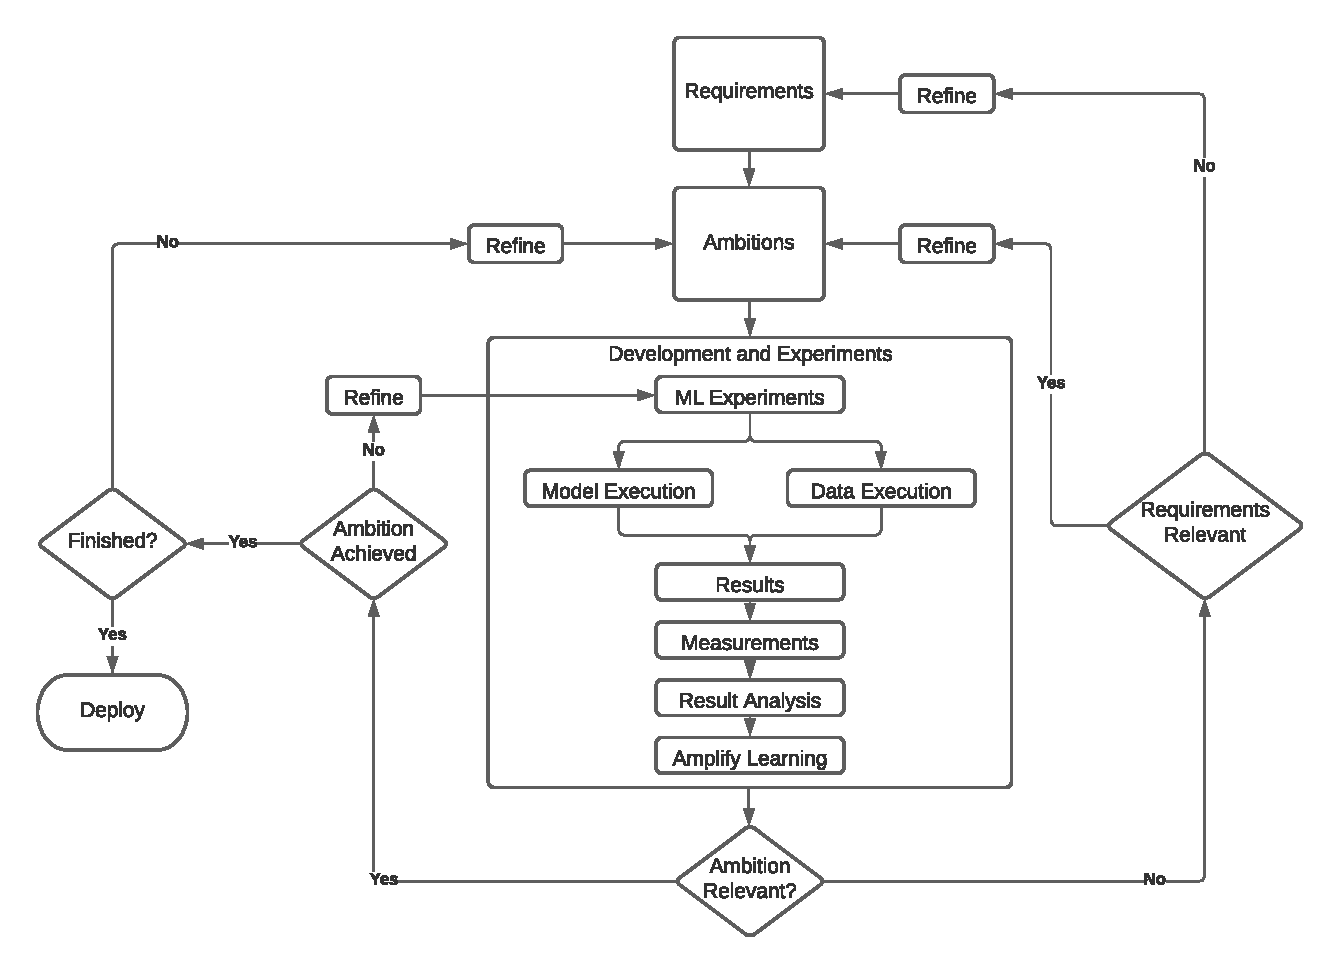
\includegraphics[width=\textwidth]{figures/chapter-3/MLDC.pdf}
    \caption[Machine Learning Development Lifecycle]{Workflow for the development of my project.
    \label{fig:MLDC}}
\end{figure}

The proposed methodology includes an Agile and Iterative core, the project requirements are directly transposed into the ML ambitions, the ML ambitions are obtained with the guidance of its experiments. This approach allows for deferred commitment with scope and requirements, code quality and coverage whilst achieving a quick artifact delivery \parencite{pinhasi2021mldc}.

\subsection{Elected SDLC}

This project strictly follows the Cross Industry Process for Data Mining model, widely known as CRISP-DM; when executing the development of a machine learning based project, there are several prefacing steps such as planning, organisation, and implementation, currently there is no standard model to efficiently carry out the development of such a project and this is where the CRISP---DM model is useful. It aims to intersect personal skills and knowledge into an effective and effective process \parencite{wirth2000crisp}. The proposed workflow can be displayed within a model such that:

\begin{figure}[H]
    \centering
    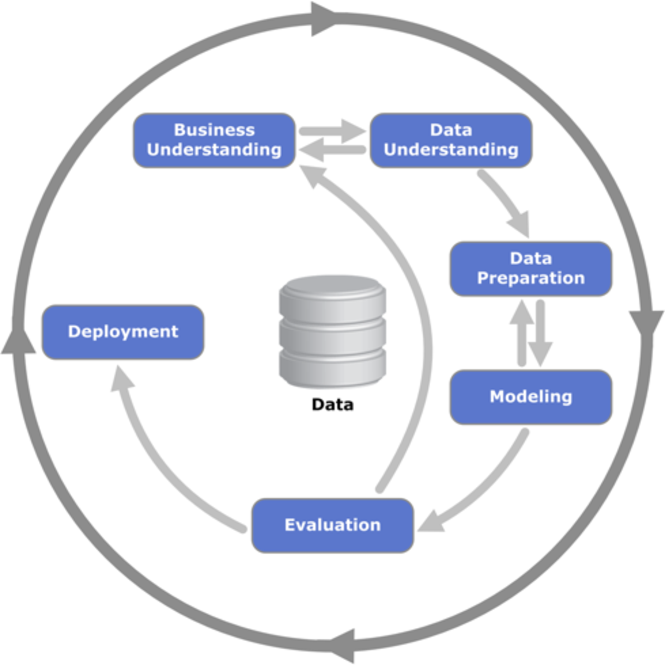
\includegraphics[width=\textwidth]{figures/chapter-3/CRISP-DM1.pdf}
    \caption[CRISP-DM Lifecycle]{The CRISP-DM Software Development Lifecycle \parencite{jenson2012crisp}.
    \label{fig:CRISP-DM}}
\end{figure}

This methodology can be described as a hierarchical process model as there is an apparent level of abstraction, being described as: phases, generic tasks, specialised tasks, and process instances \parencite{wirth2000crisp}. This process is beneficial as it can be applied to this project, each section is broken down into its respected hierarchy and labelled appropriately which is then handled in development, it allows for stable agile development as the developer can refine requirements or datasets as the project goes on, however acknowledging potential unforeseen aspects.

The process model can be deconstructed into six specific categories or phases (\autoref{fig:CRISP-DM}):

\begin{itemize}
    \item \textbf{\textit{Business Understanding}}: rather than business understanding, the context for this project is the project scope itself, the developer needs to understand the context of the problem.
    \item \textbf{\textit{Data Understanding}}: understanding the initial data collected to identify data quality and detect potential insights.
    \item \textbf{\textit{Data Preparation}}: once the initial data is collected and analysed, it will need to be prepared to construct a finalised usable dataset for the model to be parsed.
    \item \textbf{\textit{Modelling}}: this phase deals with how the data is parsed into the model after applying the intended ML techniques, this is very similar to preparation phase.
    \item \textbf{\textit{Evaluation}}: once the desired models have been constructed and the data has been parsed, it will need a quality check to ensure analysis is correct before deployment.
    \item \textbf{\textit{Deployment}}: the requirements have been met by the developer and the model yield appropriate results, the model can be deployed to an appropriate environment.
\end{itemize}

As data mining is not a standard domain which can produce varied results depending on how the project is structured and outlined, the need for a standard framework was apparent for this project. There is not reject reasoning behind this selected SDLC as the approach aims to improve accuracy, efficiency, and effectiveness of data mining applications.

\section{Project Management}

\subsection{Development Management}

The source code to this project was decided to be monitored via a GIT repository stored on GitHub; the use of version control for a machine-learning based project is especially helpful as you can backtrack certain functions that outperform changes without affecting the entire stack. The choice to use GIT opposed to a local project had several factors, such as:

\begin{itemize}
    \item Version control
    \item Track bugs
    \item Back-Up complete
    \item Branches for different features
    \item Testing purposes
    \item Source Code sharing
        \begin{itemize}
            \item Developer to supervisor
            \item Developer to developer systems
        \end{itemize}
\end{itemize}

GitHub was the chosen hosting platform due to industry standard and familiarity to both the developer and project supervisor, however, other GIT based hosting platforms such as GitLab or BitBucket do exist that satisfy the same project requirements.

\newpage

\subsection{Task Management}

Delegation of project tasks evolved over the course of completion; mentally keeping track of project TODOs became mentally taxing, thus a formal system for task delegation was implemented. As this project was completed by a sole developer, that immediately ruled out the use of a SCRUM based project board as team roles were not necessary, therefore, the “easy-to-adopt” KANBAN method was implemented, which by itself is also justification for a LEAN based SDLC model. KANBAN is a solution in which eases aspects of project design, management, improvement flow and situational knowledge and awareness by visualising (a simplified) “TODO”, “DOING”, and “DONE” categories. This in turn balances work demands compared to work capacity.

% TODO Recreate placeholders to show valid entries
This project uses two KANBAN applications, separated by general delegation and development delegation, to oversee metrics such as developer velocity, lead and time cycle, and actionable agile metrics, a Trello Board was implemented that included all tasks related to this project and report.

% Placeholder until entries are made
\begin{figure}[H]
    \centering
    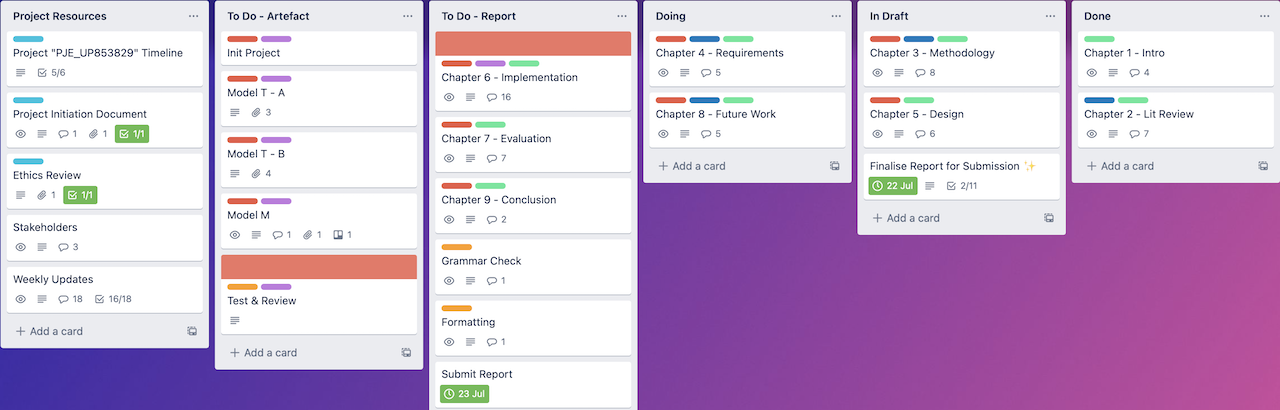
\includegraphics[width=\textwidth]{figures/chapter-3/trel.png}
    \caption[Trello Project Management KANAN Board]{Trello Project Management KANAN Board.
    \label{fig:TrelloKANBANpdf}}
\end{figure}

\newpage

In addition, a GitKraken Board was used for development related tasks such as feature ideas and bugs, these two boards were synced for a complete overview of tasks on Trello to capture the project’s work-in-progress (WIP) limits.

% Placeholder until entries are made
\begin{figure}[H]
    \centering
    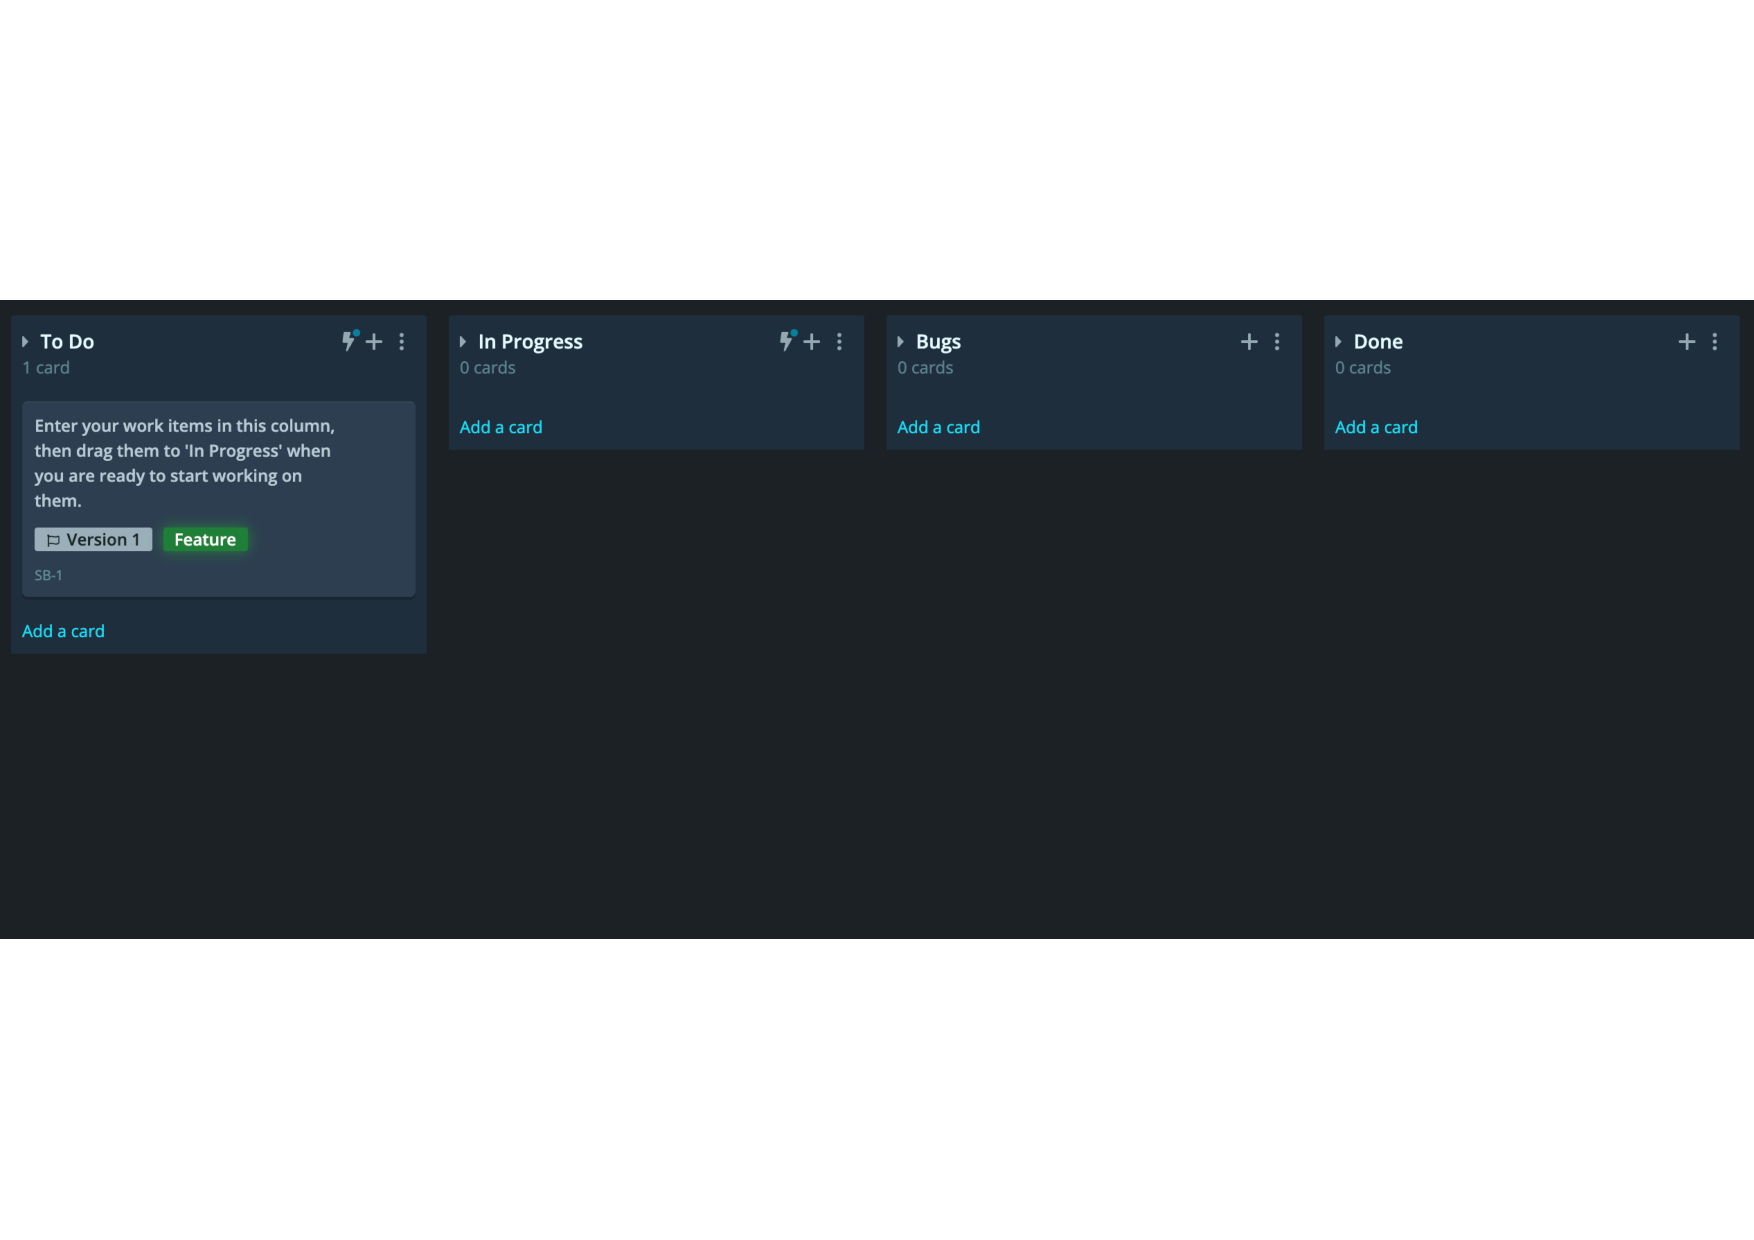
\includegraphics[width=\textwidth]{figures/chapter-3/GitKrackenKANBANpdf.pdf}
    \caption[GitKracken Development KANAN Board]{GitKracken Development KANAN Board.
    \label{fig:GitKrackenKANBANpdf}}
\end{figure}

\subsection{Time Management}

Within the Project-initiation Document (PID) in Appendix A, a Gantt Chart is supplied detailing the expected timeline this project will follow. However, it was subject to change and adaptations due to unforeseen circumstances, the below is a Gantt Chart detailing an accurate time-frame which was created nearer project end:

% TODO Remake Gantt Chart to dislay an accurate timeline
\begin{figure}[H]
    \centering
    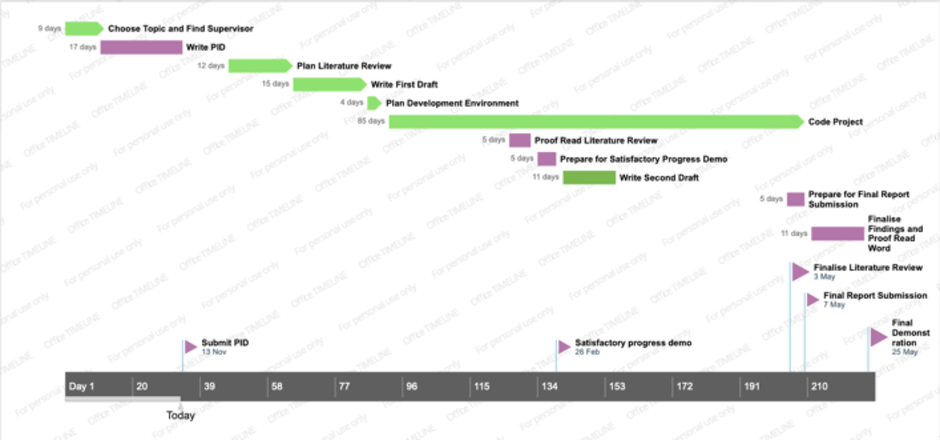
\includegraphics[width=\textwidth]{figures/chapter-3/ProjectGanttChart.pdf}
    \caption[Project Gantt Chart]{Project Gantt Chart.
    \label{fig:ProjectGanttChart}}
\end{figure}

\chapter{Requirements and Planning}

This chapter outlines the desired requirements which are necessary for this project to work and to have met the criteria proposed, it also includes additional requirements such as potential requirements and unnecessary but topical requirements. In section 3.1.3, the model flowchart displays requirements must be detailed as part of the SDLC for project ambitions and solution scope; all requirements listed are relevant to a machine learning NLP focused model, seen as a process orientated requirement.

\section{Requirement Elicitation}

Requirement elicitation for this project started by defining its scope, planning a potential solution and desired outcome to further have a discussion with the project supervisor, to gain requirement insight. The project’s functionality and capabilities were outlined in-order for the functional and non-functional requirements to be identified.

As no human parties were involved, other than the developer and project supervisor, no external input was involved. Therefore, the requirement elicitation process primarily focused on academic research and existing applications of similar intent. Existing text classification machine learning models provided insight to potential requirements; the research covered in the literature review (section 2) under existing applications highlighted key areas of interest. This project benefitted from deriving requirements seen from a process perspective opposed to traditional methods such as a questionnaire, for example a procedural step within the machine-learning process i.e., model must clean data.

\subsection{Requirement Research of Current Models}

This project's system and functional requirements can be broken down into a simplified structure, such that the procoess for text classification if as follows:

\begin{enumerate}
    \item Parse Data
    \item Pre-processing of Data
    \begin{enumerate}
        \item Tokenization
        \item Vectorization
    \end{enumerate}
\item Text pre-processing
\item Clean data
    \begin{enumerate}
        \item Remove empty data, useless punctuation, and unnecessary stop words
        \item Stem the words
    \end{enumerate}
\item Feature Engineering and Extraction
\item Feed clean dataset into model
\item Train model
\item Tune hyper-parameters
    \begin{enumerate}
        \item Number of layers in model and units per layer
        \item Dropout rate
        \item Learning rate
        \item Kernel size
        \item Embedding
    \end{enumerate}
\item Evaluate model
\end{enumerate}

\section{Requirement Specification}

This project makes use of the MoSCoW prioritisation technique whereby requirements are defined as “Must Have”, “Should Have”, “Could have”, and “Won’t Have at this Time”. The four categories of MoSCoW can be translated to Core, Base, Additional, and Future Work. This project acknowledges the disadvantages of the MoSCoW technique; however, its simplicity outweighs the disadvantages in this environment.

\section{Requirement Constraints}

\begin{itemize}
    \item Issues locating appropriate openly sourced datasets of existing student feedback.
    \item Accuracy of model given located datasets.
    \item Components of the model may not communicate well with other aspects.
    \item Programming and language concern.
    \item Logistical issues.
\end{itemize}

Defining potential constraints of this project aided identifying its functional and non-functional requirements as there was an insight as to what may work or not work when in the development phase, these requirements are listed below with the appropriate level of prioritisation.

\section{Functional Requirements} \label{section:FunctionalRequirements}

\begin{itemize}
    \item \textbf{\textit{Must Have}}
        \begin{itemize}\label{FMH}
            \item MH1
            \item The model must correctly parse a given dataset such that the correctness of the original dataset is intact.
            \item The model must pre-process the dataset into a given method: tokens/vectors.
            \item The model must pre-process the text within the dataset into specific categories.
            \item The model must clean the text such that cleaning involves the removal of empty fields within a CSV file, any useless or incorrect punctuation, and unnecessary stop words.
            \item The model must take the clean data and categories stem words.
            \item The model must produce a machine learning implementation that learns and is trained on sample data that is then extrapolated into a useable asset.
            \item The model must classify text.
        \end{itemize}
    \item \textbf{\textit{Should Have}}
        \begin{itemize}\label{FSH}
            \item SH1
            \item The model solution should be agnostic towards data types, data sensors, vendor (mostly universities or colleges) and data creation date.
            \item The model should report analysis in real-time with graphs or training data within the CLI, this includes any abnormalities which might need deeper analysis to be useful data.
            \item The model must execute statistical analysis on the yielded information which is generated for future examination.
        \end{itemize}
    \item \textbf{\textit{Could Have}}
        \begin{itemize}\label{FCH}
            \item CH1
            \item The model could provide an analytical solution in which communicates with processing features.
            \item The model could create an interactable alert so the user can decide on how to proceed.
            \item The model may predict future student evaluations.
            \item The model could save outputted data to a local text file
            \item The model could have param-arguments for it's runtime, most likely in the form of CLI arguments, this allows the model to execute commands in a certain order, i.e \verb-----parse to select the input dataset.
        \end{itemize}
    \item \textbf{\textit{Won't Have}}
        \begin{itemize}\label{FWH}
            \item WH1
            \item The model won’t have a GUI (can be developed for future work).
        \end{itemize}
\end{itemize}

\section{Non---Functional Requirements} \label{section:NonFunctionalRequirements}

\begin{itemize}
    \item \textbf{\textit{Must Have}}
        \begin{itemize}\label{NFMH}
            \item MH1
            \item The model must provide and produce an accurate F-Score.
            \item The model must be maintainable within its set scope, overdeveloping or under developing can lead to bugs or broken links such as outdated APIs.
        \end{itemize}
    \item \textbf{\textit{Should Have}}
        \begin{itemize}\label{NFSH}
            \item SH1
            \item The model may yield predictions or results limited to the scope of a set asset.
            \item The model may yield results across several datasets.
            \item The model must yield maximum theoretical performance for its implementation, this includes:
                \begin{itemize}
                    \item Correct potential true positives
                    \item Correct potential false positives
                    \item Account for and correct false negatives
                    \item Recall of data and specifics
                \end{itemize}
            \item The model should yield optimal precision of data and classification.
            \item The model should run within an acceptable time-frame for a given machine, e.g., testing must not run over 24hrs for an appropriate dataset.
            \item The should must be useable for a lay person who wants to classify text (school admin).
        \end{itemize}
    \item \textbf{\textit{Could Have}}
        \begin{itemize}\label{NFCH}
            \item CH1
            \item The model may be scalable for multiple datasets or machines.
        \end{itemize}
    \item \textbf{\textit{Won't Have}}
        \begin{itemize}\label{NFWH}
            \item WH1
        \end{itemize}
\end{itemize}

\section{Challenges in Requirements}

Challenges

\section{Cost Prediction}

This project will not have any costs associated with or throughout the development. However, future development may include renting server space for better spec machines to run training of this model.
% \chapter{Project Design}

This chapter outlines the design behind each component of the NLP model and the respected process each component may entail, several components will execute more than one step to achieve the desired result. The design is reflected within the final model and each component is broken down to display the functionality and theory within this project. Within section \ref{section:FunctionalRequirements}, it is detailed there won’t be a GUI for the interaction and thus the design section relates to the inner workings of the model itself, that being: system architecture, logistics and theory.

\section{Classical vs Modern}

As originally intended, this project would have seen two differing implementations of the same concept, one being of a classical nature and the other being a machine learning variation, as previously mentioned this project experienced time management issues due to unexpected issue, to which resulted in only focusing on the machine learning implementation of a novel approach. The design for the first model would have been of the following:

\begin{figure}[H]
    \centering
    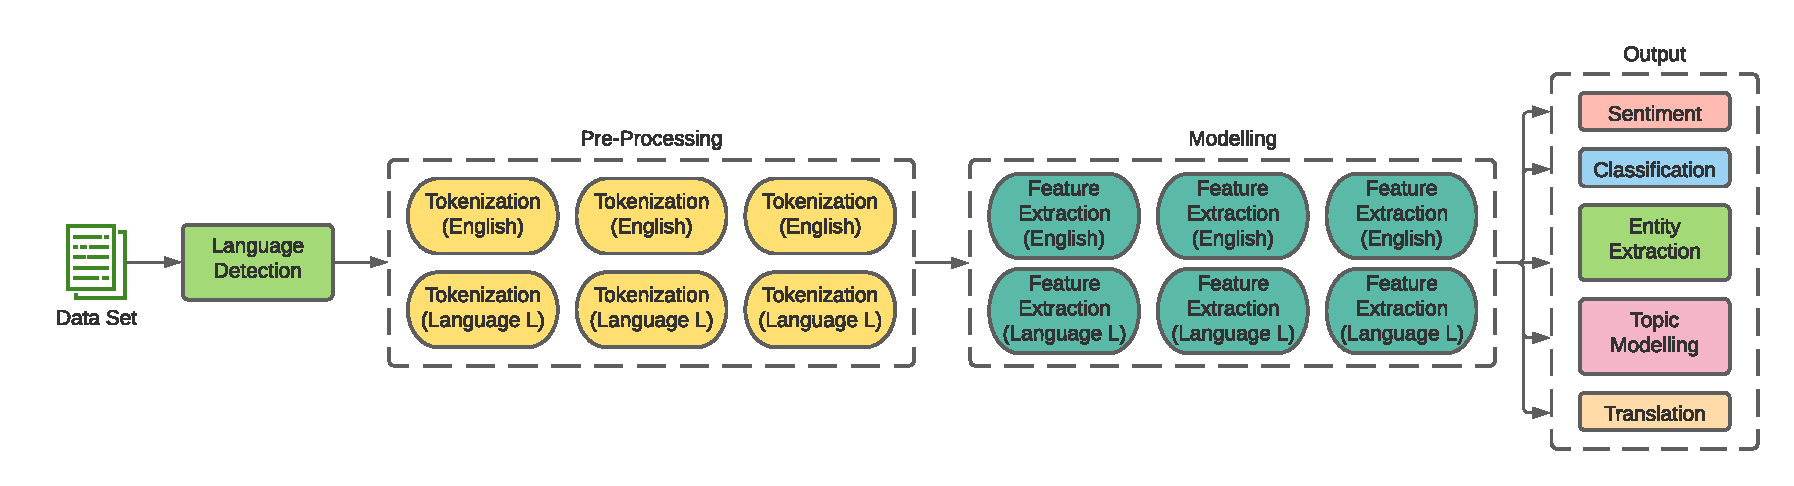
\includegraphics[width=\textwidth]{figures/chapter-5/ClassicalNLP.pdf}
    \caption[ClassicalNLP]{Classical NLP pipeline for text classification.
    \label{fig:ClassicalNLP}}
\end{figure}

Classical or traditional methods for NLP include: N-Gram, Hidden Markov Models using Markov Chains and Part-Of-Speech Tagging. The developer had originally intended to implement a traditional approach within a machine learning model. The combination of Part-Of-Speech with a machine learning model to calculate a word’s vector based on its TF-IDF value would have been the start, such that:

\begin{equation}
    tf(t,d) = \frac{f_t, _d}{\sum{t \in_d} f _t {_`}, _d}
\end{equation}

It would have also used the inverse TF-IDF value as the project model covers multiple datasets, such that:

\begin{equation}
    idf(t, D) = \log \frac{N}{|d \in D : t \in d|}
\end{equation}

Where the traditional aspect of the Bag-of-Words would produce a vector for each item in a corpus, it’s TF-IDF value would have been calculate through a series of CNN nodes.

Machine learning concepts can be classed as a “black-box” of functionality as the user does not necessarily see what is being executed within the hidden layers, a high-level abstraction for this project can be generalised into the following diagram:

\begin{figure}[H]
    \centering
    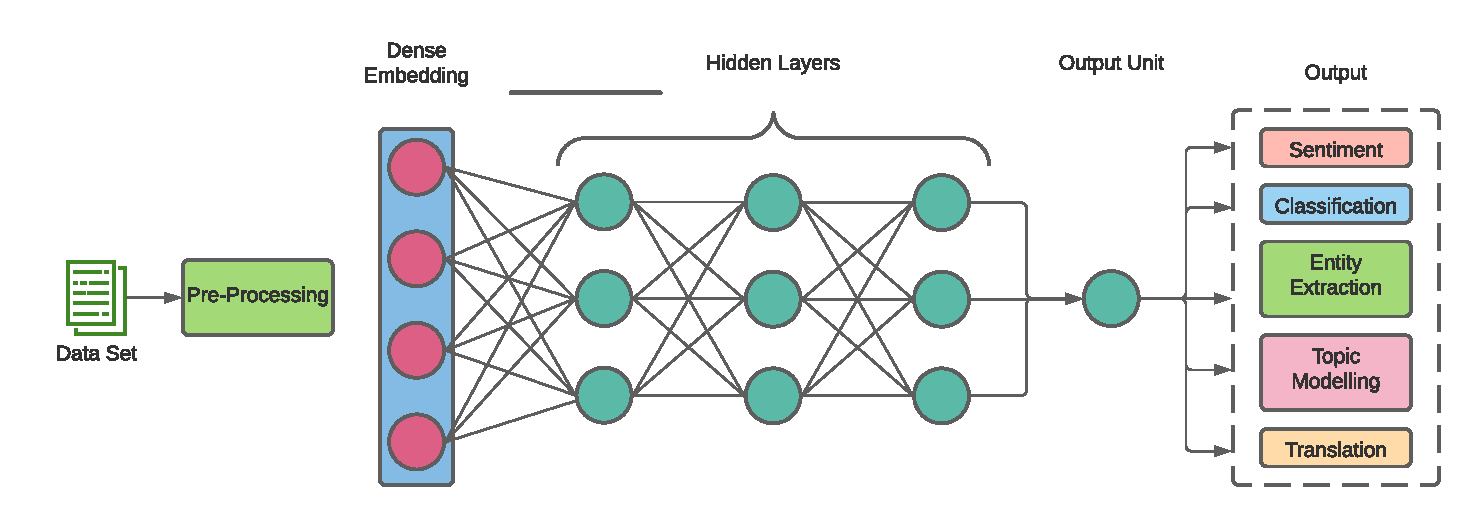
\includegraphics[width=\textwidth]{figures/chapter-5/MLNLP.pdf}
    \caption[MachineLearningNLP]{Machine Learning Model for an NLP pipeline for text classification.
    \label{fig:MLNLP}}
\end{figure}

\section{Planning the ML Model Design}

Initial prototyping of the machine learning model for a new amalgamation of NLP techniques helped to indicate what the best route of development could be, the planning stage piggybacked off existing work flowchart diagrams in-order to choose the most appropriate method and technique combination. The sequence flowchart is as follows:

\begin{figure}[H]
    \centering
    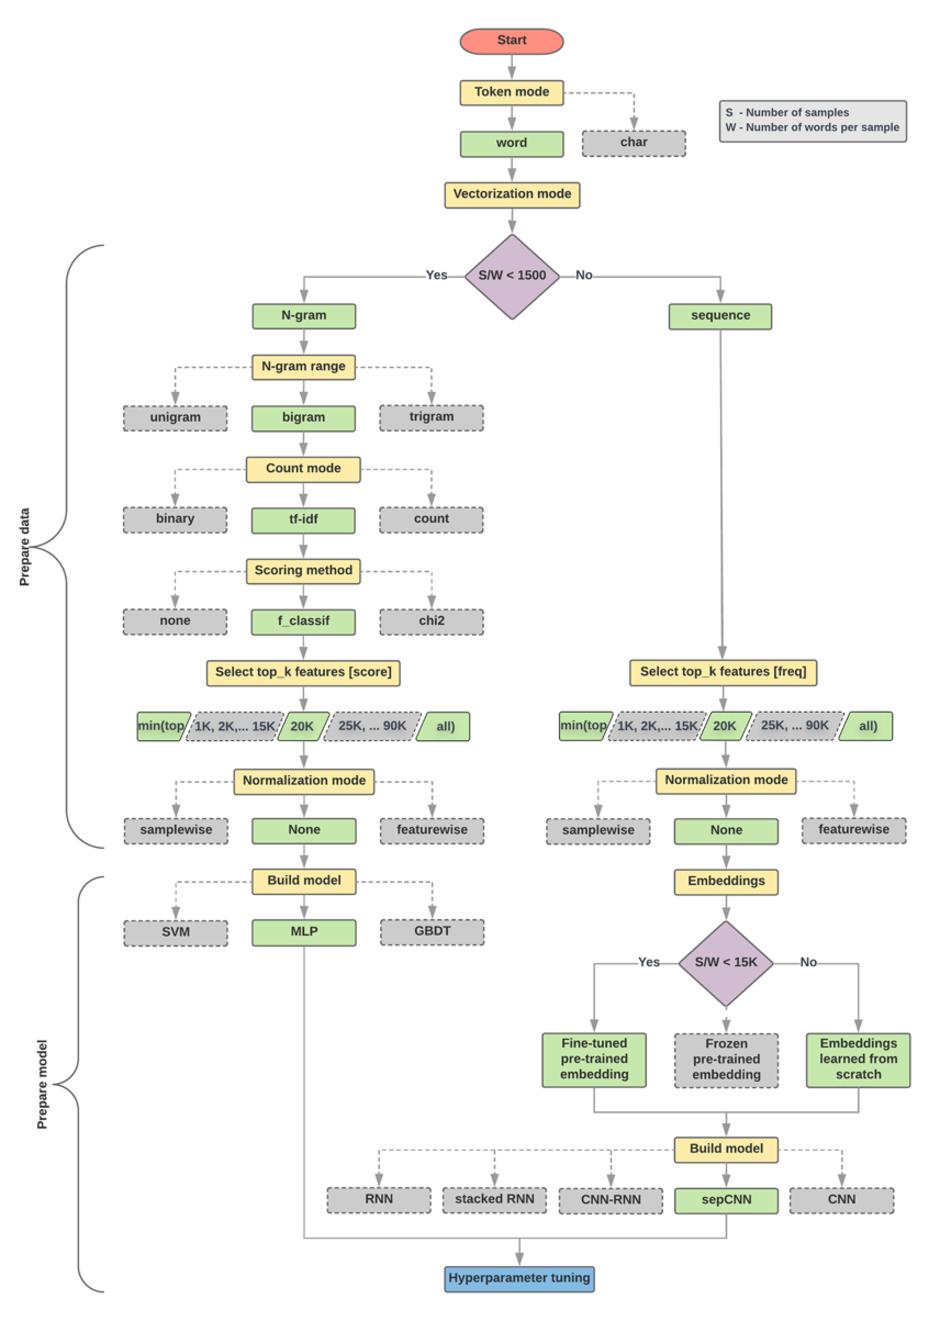
\includegraphics[width=\textwidth]{figures/chapter-5/GooglePlan.pdf}
    \caption[GooglePlan]{Text Classification Flowchart \parencite{google2021TCF}.
    \label{fig:GooglePlan}}
\end{figure}

\section{Supervision}

The development of the project model is based on a supervised approach due to the datasets located, it was most appropriate to use a supervised approach due to the datasets having no labels or lexical categories to train the model on; the model has user input to account for missing labels on data which have been manually and algorithmically added. The supervision for this project can be represented as the following diagram:

\begin{figure}[H]
    \centering
    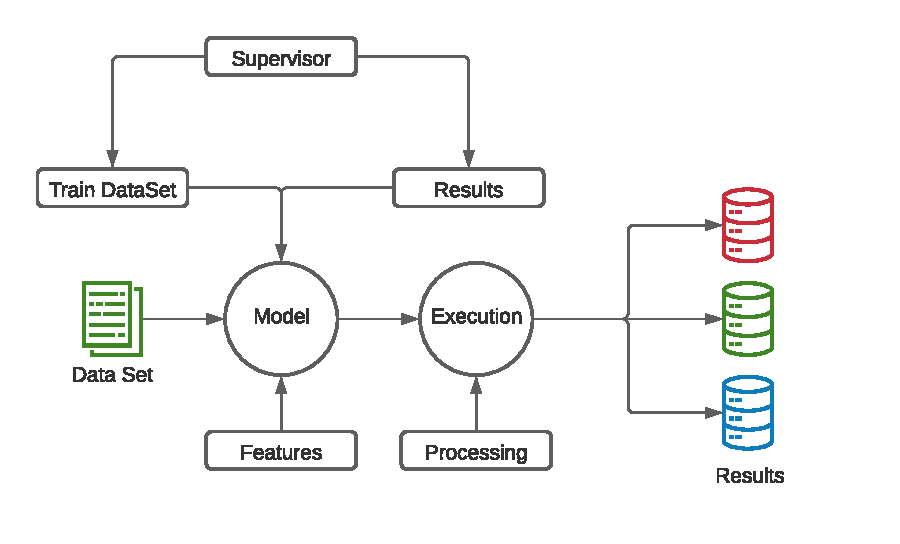
\includegraphics[width=\textwidth]{figures/chapter-5/SupervisedLearningChart.pdf}
    \caption[SupervisedLearning]{Sequence control for Supervised learning.
    \label{fig:SupervisedLearningChart}}
\end{figure}

\section{Pipeline Design}

\begin{figure}[H]
    \centering
    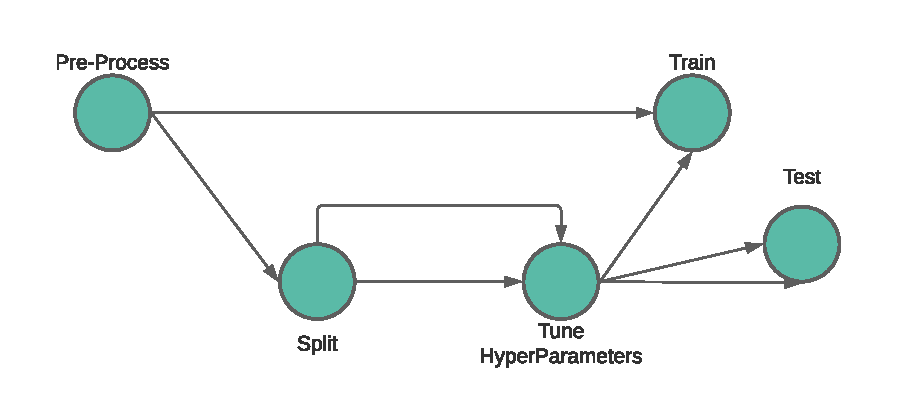
\includegraphics[width=\textwidth]{figures/chapter-5/Pipeline.pdf}
    \caption[MLTCPipeline]{Pipeline for model classification.
    \label{fig:MLTCPipeline}}
\end{figure}

There are five main steps for a text classification pipeline:

\begin{enumerate}
    \item \textbf{\textit{Pre-processing}}: prepare the raw dataset to be trained.
    \item \textbf{\textit{Splitting}}: split the processed dataset to be trained and validated.
    \item \textbf{\textit{Tuning}}: identity valuable parameters within trained data.
    \item \textbf{\textit{Training}}: train the current iteration of the model with updated hyper-parameters.
    \item \textbf{\textit{Testing}}: test and collect statistics for analysis to make further predictions.
\end{enumerate}

\section{Data Preparing and Pre---processing}

Data Preparing

\section{Model}



Skip-gram rather than (Continuous)Bag-Of-Words (CBOW) as it yields better results with large datasets - such as student feedback - skip gram can also be context aware as it converts neighboring lexemes to vectors

\subsection{Skip-Gram}

\begin{figure}[H]
    \centering
    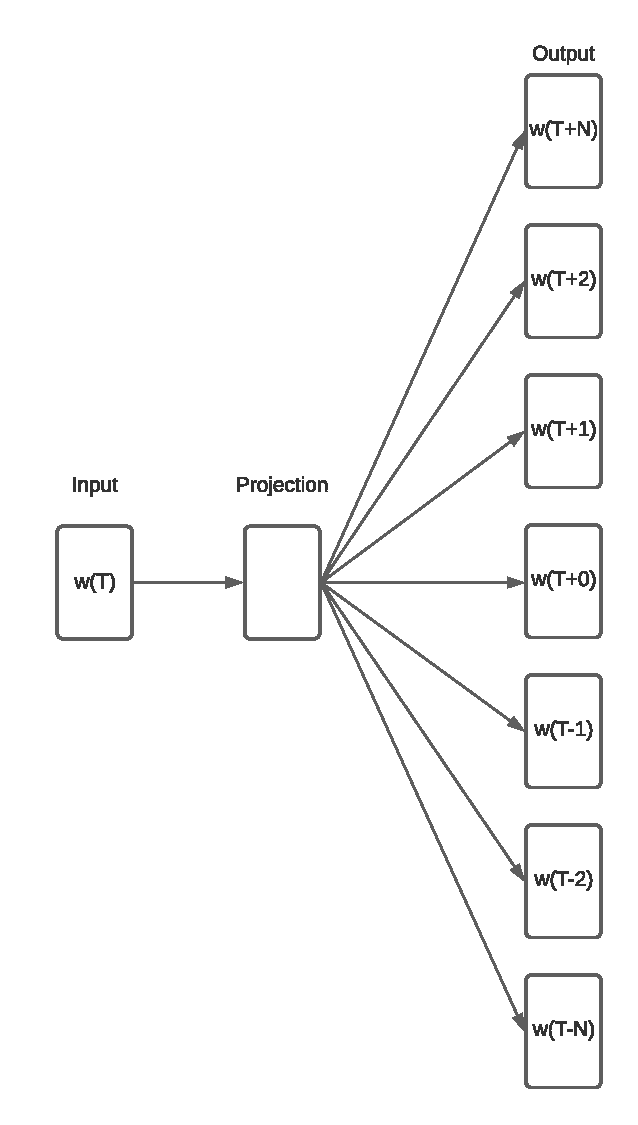
\includegraphics[width=0.49\textwidth]{figures/chapter-5/SkipGramModel.pdf}
    \caption[SkipGramModel]{Input flow of Skip-Gram model.
    \label{fig:SkipGramModel}}
\end{figure}

The skip-gram model can be seen as the inverse of the bag-of-words model as it attempts to vectorize neighboring words first to identify corpus context, whereas, bag-of-words takes each lexeme first, produces a vector sum and then categorises each word.

% https://machinelearningmastery.com/gentle-introduction-bag-words-model/
% https://towardsdatascience.com/pos-tagging-using-crfs-ea430c5fb78b#1c6a

\subsection{The Artefact}

POS TAGGING + Machine Learning

"POS tags are another way of labeling text data, in particular we are labeling the to- kens/words in a text. ... In a way POS tags are in themselves features of words; they give classification and context to words that allow us to better understand the purpose of word choice and the meaning of sentences as a whole."
\chapter{Project Design - New} \label{chapter:ProjectDesign}

This chapter outlines the design behind each component of the text classification model and the respected process each component may entail, several components will execute more than one step to achieve the desired result. The design is reflected within the final model and each component is broken down to display the functionality and theory within this project. In \autoref{section:FunctionalRequirements}, it is detailed there won’t be a GUI for the interaction and thus the design section relates to the inner workings of the model itself, that being: system architecture, logistics and theory.

\section{Classical vs Modern}

As originally intended, this project would have demonstrated two differing implementations of the same concept, one being of a classical nature implemented as a machine learning model and the other being a modern variation of the same approach, as previously mentioned this project experienced time management issues due to unexpected problems, to which resulted in only focusing on a traditional implementation within a modern model in attempt at a novel approach. \newpage

Classical NLP implementations can be described as:

\begin{figure}[H]
    \centering
    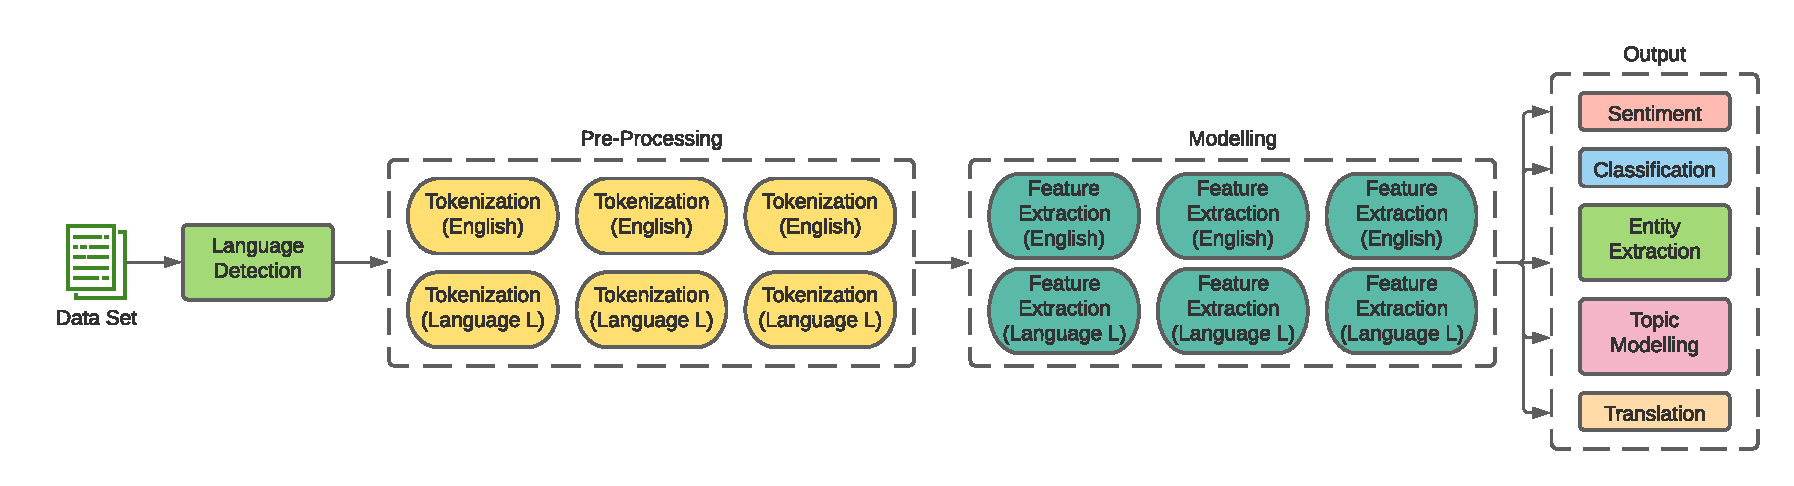
\includegraphics[width=\textwidth]{figures/chapter-5/ClassicalNLP.pdf}
    \caption[ClassicalNLP]{Classical NLP pipeline for text classification.
    \label{fig:ClassicalNLP}}
\end{figure}

Classical or "traditional" methods for corpus classification include: N-Grams, Hidden Markov Models using Markov Chains, Part-Of-Speech Tagging and Bag-Of-Words. Machine learning concepts can be classed as a “black-box” of functionality as the user does not necessarily see what is being executed within the hidden layers, a high-level abstraction for this project can be generalised into the following diagram:

\begin{figure}[H]
    \centering
    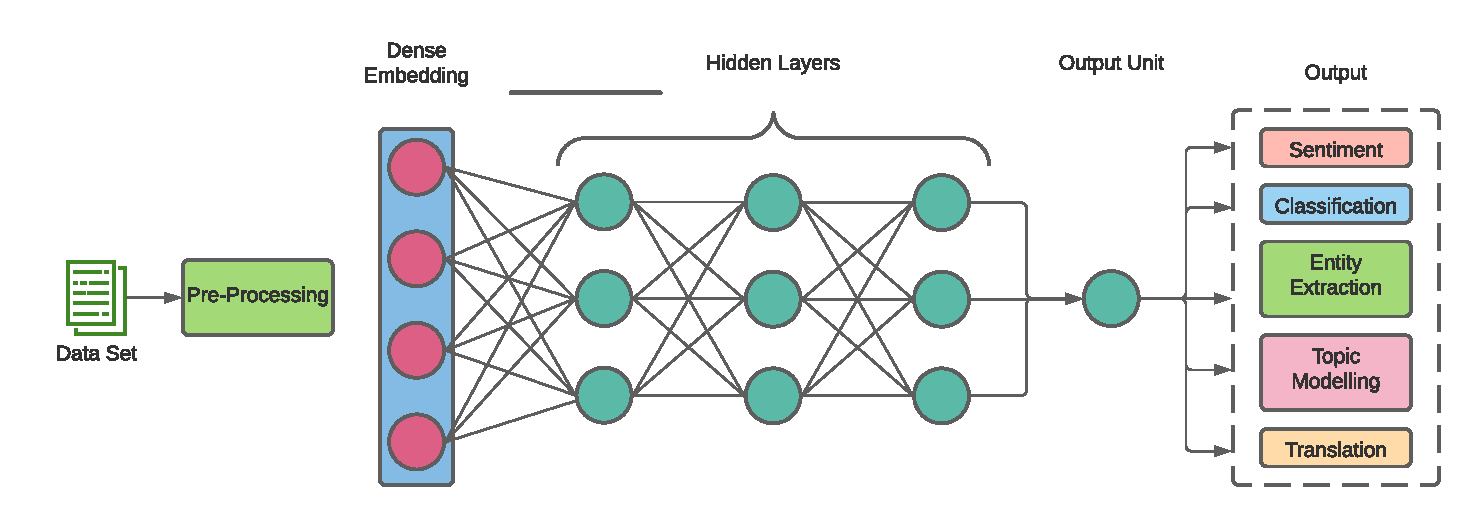
\includegraphics[width=\textwidth]{figures/chapter-5/MLNLP.pdf}
    \caption[MachineLearningNLP]{Machine Learning Model for an NLP pipeline for text classification.
    \label{fig:MLNLP}}
\end{figure}

\section{Model Approach --- Traditional (A)} \label{sub:C5ModelATraditionalA}

The traditional implementation would have been designed based on word-embeddings within a 2D space where word vector values would be used alongside the Bag-Of-Words approach. The combination of Bag-Of-Words with a machine learning model to calculate a word’s vector based on its TF-IDF value would have been the start, such that:

\begin{equation}
    tf(t,d) = \frac{f_t, _d}{\sum{t \in_d} f _t {_`}, _d}
\end{equation}

Where the TF-IDF value is how often a lexeme occurs in a given corpus and would have also used the inverse TF-IDF value as the project model covers multiple datasets, such that:

\begin{equation}
    idf(t, D) = \log \frac{N}{|d \in D : t \in d|}
\end{equation}

Where the inverse TF-IDF value is represents how rare a word is in a given corpus.

\subsection{Limitations of Bag-Of-Words}

As there is a specific domain for this project, it is important to focus on the limitations for potential methods, BOW models have demonstrated high training accuracy and is a relatively simple model to implement, it is naturally flexible as it can be trained on different datasets for a specific context; however, it does have disadvantages for classification and text prediction. Universities host students from different backgrounds and levels of education which can imply issues when training datasets, these issues can impact:

\begin{itemize}
    \item \textbf{\textit{Vocabulary:}} Students may have varying output to describe the same context, this can create confusion for training.
    \item \textbf{\textit{Frequency:}} The frequency of a word may influence its power in a dataset.
    \item \textbf{\textit{Context:}} If students describe the same situation in a different way, some words may lose semantic meaning or be interpreted incorrectly, for example isolating neologisms, synonyms, colloquialism, polysemes, or semantic change.
\end{itemize}

As a result, the Bag-Of-Words approach is not considered for this comparison for the domain of student feedback analysis.

\section{Model Approach --- Traditional (B)} \label{sub:C5ModelATraditionalB}

POS---TAGGING

\section{Model Approach --- Modern}

Modern or "contemporary" methods for corpus classification include: \ldots The modern implementation would have been based around Word2Vec implemented in a machine learning model for Sentiment Analysis which can be seen as a subcategory of text classification. The word2vec implementation would produce vector values for identified key words and plot them as such:

\begin{figure}[H]
    \centering
    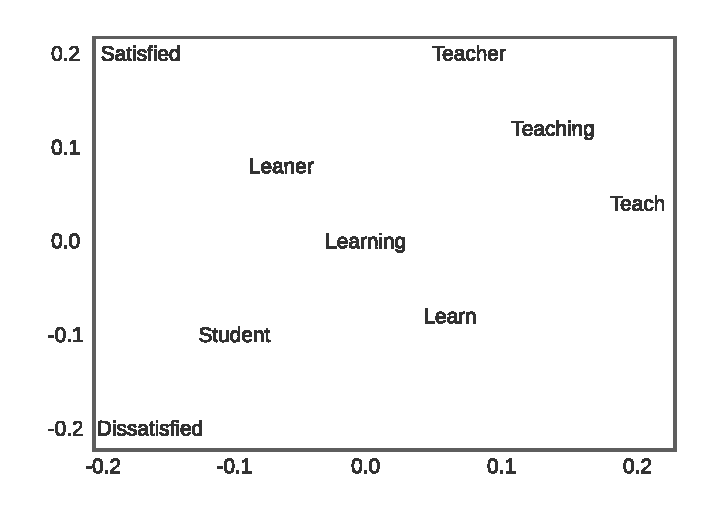
\includegraphics[width=\textwidth]{figures/chapter-5/Example-Word-Vector.pdf}
    \caption[ExampleWordVector]{Example of student satisfaction vector graph in 2d space.
    \label{fig:Example-Word-Vector}}
\end{figure}

\subsection{Word2Vec Skip-Gram} \label{sub:Word2VecSkipGram}

Skip-gram rather than Continuous Bag-Of-Words (CBOW [which is the modern implementation of Bag-Of-Words]) as it yields better results with large datasets - such as student feedback - skip gram can also be context aware as it converts neighboring lexemes to vectors.

\begin{figure}[H]
    \centering
    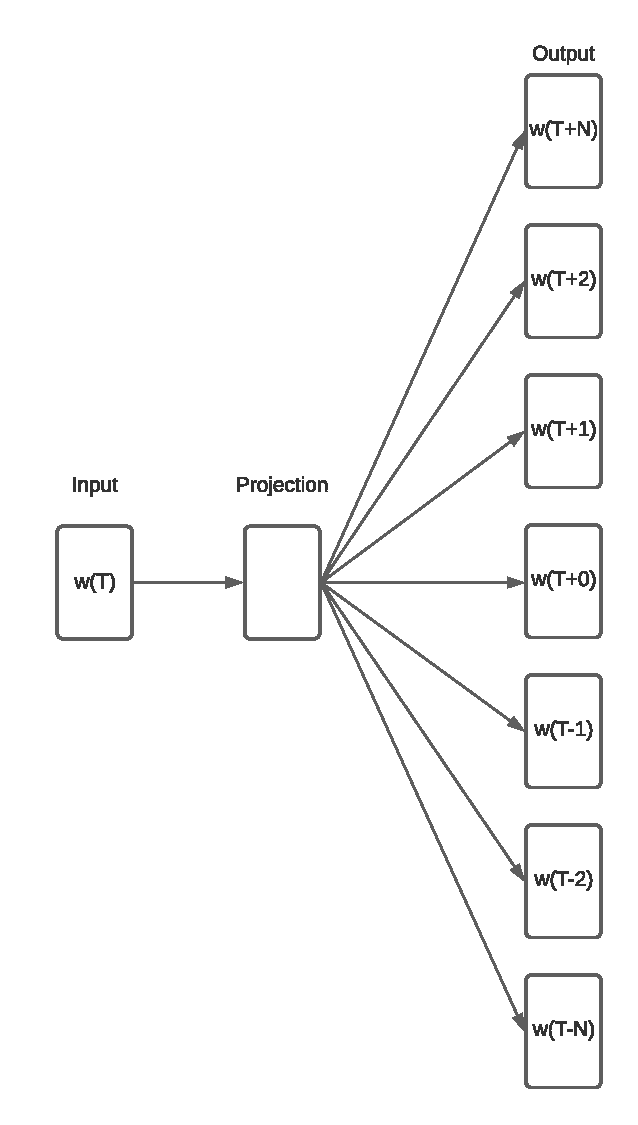
\includegraphics[width=0.49\textwidth]{figures/chapter-5/SkipGramModel.pdf}
    \caption[SkipGramModel]{Input flow of Skip-Gram model.
    \label{fig:SkipGramModel}}
\end{figure}

The skip-gram model can be seen as the inverse of the bag-of-words model as it attempts to vectorize neighboring words first to identify corpus context, whereas, bag-of-words takes each lexeme first, produces a vector sum and then categorises each word. \newpage

The Skip-Gram's network architecture is similar to the diagram displayed in \autoref{fig:MLNLP}, the diagram above is another level of abstraction as to how this project will make use of machine learning fundamentals.

\begin{figure}[H]
    \centering
    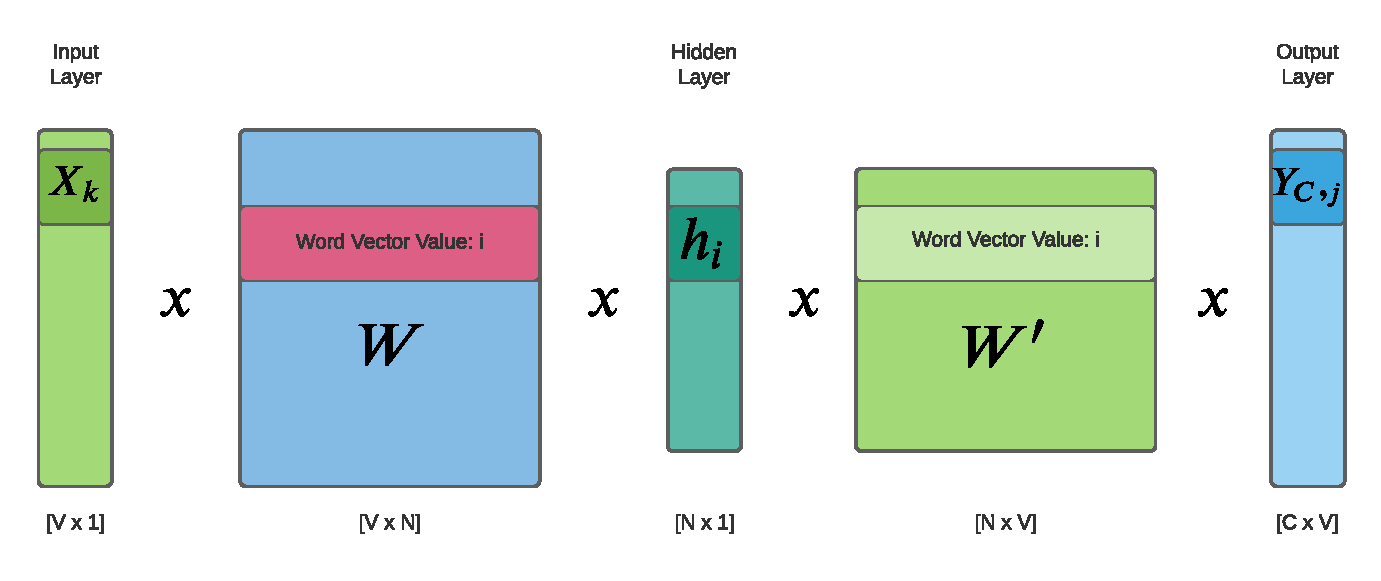
\includegraphics[width=\textwidth]{figures/chapter-5/SkipGramNetwork.pdf}
    \caption[SkipGramNetwork]{Skip-Gram implementation for Word2Vec network architecture.
    \label{fig:SkipGramNetwork}}
\end{figure}

\subsection{One-Hot Encoding} \label{sub:Word2VecOneHotEncoding}

Encoding each significant lexeme in a given dataset is helpful for the model to distinguish the level of importance, outlined as context, the diagram shown above in \autoref{fig:SkipGramModel} takes a 1D row vector as the input layer which allows for the model to acceptably one-hot encode each lexeme unit as a numeric value.

\begin{multicols}{2}
    \begin{equation*}
        "Teach" =
        \begin{bmatrix}
            0, & 0, & 0, & 0, & 1, & 0
        \end{bmatrix}
    \end{equation*}

    \begin{equation*}
        "Teaching" =
        \begin{bmatrix}
            0, & 0, & 0, & 0, & 1, & 0
        \end{bmatrix}
    \end{equation*}
\end{multicols}

This equates to differing versions of the same word (root + free or bound morpheme [affix]) to have the same influence when being parsed forward within the training model.

\subsection{Forward Propagation} \label{sub:Word2VecForwardPropagation}

Once the corpus text is encoded as an acceptable 1D matrix, it can then be parsed to the first hidden layer's node:

\begin{equation}
    h = x^T W
\end{equation}
`x' represents the row vector, `h' can be taken as the column height ($[x]^T$ of the vector `W' where `h' is the `$k_{th}$' column.

\begin{equation}
    h = W_{(k,:)}^{T} \coloneqq v_{w_I}^{T}
\end{equation}
As each lexeme unit parses through the hidden layer nodes, the exit value needs to be calculated:

\begin{equation} \label{eq:u_cDefinition}
    u_{c} = W'^{T}h = W'^{T} W^{T}x
\end{equation}
For simplicity, $u_{c}$ will transpose each unit through the model in its entirety, however, the value(s) of $u_{c}$ cause performancy and memory issues in the model. Thus, \textbf{\textit{softmax}} will be used to slice the vector value of $u_{c}$ to [0,1].

\begin{equation*}
    y_{c} = Softmax(u)
\end{equation*}

\begin{equation}
    p(w_{c,_j} = w_{O,_c} | w_{I}) = y_{c,_j} = \frac{exp(u_{c_,j})}{\sum_{j' = 1}^{V} exp(u_{j'})}
\end{equation}
`x' represents the center word $w(T)$ of a vector where $W'$ will yield the softmax value of $u_{c}$, this ensures the vector of $w(T)$ will have exact values of input for `x', where:

\begin{multicols}{2}
    \begin{equation*}
        u_{c,_j} = u_{j} = {v'_{w_j}} ^ T \cdot h
    \end{equation*}

    \begin{equation}
        % TODO rewrite mathematically in set theory notation
        c=1 \ldots |C|
    \end{equation}
\end{multicols}
${v'_{w_j}}$ represents the exit vector for the $j^{th}$ lexeme unit in $w_{j}$ (the corpus vocabulary).

\subsection{Backward Propagation} \label{sub:Word2VecBackardPropagation}

As stated above in \autoref{eq:u_cDefinition}, the transposition of each unit $u_{c}$ is simple where node weight is not considered. To account for the weight of the model matrices $W$ and $W'$, the Stochastic Gradient Descent method is applied, which in turn will optimise the backward propagation of node errors; when training the model, errors are bound to occur, to which a loss function is needed to calculate each layers efficiency.

\begin{equation}
    \begin{split}
        Error (E) & = - \log \mathbb{P} (w_{O_,{_1}} , \ldots, w_{O_{,c}} | w_{I}) \\
                  & = - \log \prod_{c=1}^{C} \frac{exp(u_{c,j_{c}^{*}})}{\sum_{j'=1}^{V} exp(u_{j'})}  \\
                  & = - \sum_{c=1}^{C} u_{j_{c}^{*}} + C \cdot \log \sum_{j'=1} ^ {V} exp(u_{j'})
    \end{split}
\end{equation}
${j_{c}^{*}}$ represents the exit vector column's index within the vector's vocabulary. Once loss is calculated, the model can apply the \textbf{\textit{chain rule}} for weight error classification within $W$ and $W'$. This is achieved by obtaining the partial derivative of Error(E) of each exit node $u_{c,_j}$.

\begin{equation}
    \frac{\partial E}{\partial u_{c,_j}} = y_{c,_j} - t_{c,_j} \coloneqq e_{c,_j}
\end{equation}
$t_{c,_j}$ represents vector $u$'s \textbf{\textit{Ground Truth}}; [$t_{c,_j}$]'s state of hypothesis can be represented as the following definition:

\begin{equation}
    EI_j = \sum_{c=1}^{C} e_{c,_j} = \sum_{c=1}^{C} (y_{c,_j} - t_{c,_j}) = \frac{\partial E}{\partial u_{j}}
\end{equation}
$EI_{j}$ represents the \textbf{\textit{Row-Wise Sum}} as a column vector in attempt to account for word context errors for $w(T)$; \textbf{\textit{backpropagation}} can then occur by obtaining the partial derivative of Error(E) within matrix $W'$.

\begin{equation} \label{}
    \begin{split}
        \frac{\partial E}{\partial w'_{ij}} & = \sum_{c=1}^{C} \frac{\partial E}{\partial u_{c_{,j}}} \cdot \frac{\partial u_{c_{,j}}}{\partial w'_{i_{,j}}} \\
                                            & = \sum_{c=1}^{C} (y_{c,_j} - t_{c,_j}) \\
                                            & = EI_{j} \cdot h_{i}
    \end{split}
\end{equation}
When backpropagation occurs, the Stochastic Gradient Descent is redefined in terms of the matrix $W'$:

\begin{equation}
    w'^{(new)}_{i,j} = w'^{(old)}_{i,j} - \eta \cdot EI_{j} \cdot h_{i}
\end{equation}
$\eta$ represents the model's training (learning). Once the learning rate has been established, the model can update the distribution of errors between the model layers, particularly between unit input and the hidden layer whereby the partial derivative is weighted against an error from a hidden layer. This can be calculated with:

\begin{equation}
    \begin{split}
        \frac{\partial E}{\partial h_{i}} & = \sum_{j=1}^{V} \frac{\partial E}{\partial u_{j}} \cdot \frac{\partial u_{j}}{\partial h_{i}} \\
                                          & = \sum_{j=1}^{V} EI_{j} \cdot w'_{ij}
    \end{split}
\end{equation}
As errors are calculated between the input layer and the hidden layer accounting for error weight, it is possible to calculate the weighted loss of matrix $W$ by taking the partial derivatives of Error(E) against the partial derivative of an index within matrix $W$, as such:

\begin{equation} \label{}
    \begin{split}
        \frac{\partial E}{\partial W_{ki}} & = \frac{\partial E}{\partial h_{i}} \cdot \frac{\partial h_{i}}{\partial w_{ki}} \\
                                           & = \sum_{j=1}^{V} EI_{j} \cdot w'_{ij} \cdot x_{k}
    \end{split}
\end{equation}
The weight of the Stochastic Gradient Descent is redefined in terms of the matrix $W$:


\begin{equation}
    w^{(new)}_{i,j} = w^{(old)}_{i,j} - \eta \cdot \sum_{j=1}^{V} EI_{j} \cdot w'_{ij} \cdot x_{j}
\end{equation}
The fundamental functionality has been outlined in theory but in practice will be enough to train the given Skip-Gram Network in \autoref{fig:SkipGramNetwork}.

\section{Planning the Network Architecture}

Initial prototyping of the machine learning model for a new amalgamation of NLP techniques helped to indicate what the best route of development could be, the planning stage piggybacked off existing work flowchart diagrams in-order to apply the most appropriate method and technique combination. The sequence flowchart is as follows:

\begin{figure}[H]
    \centering
    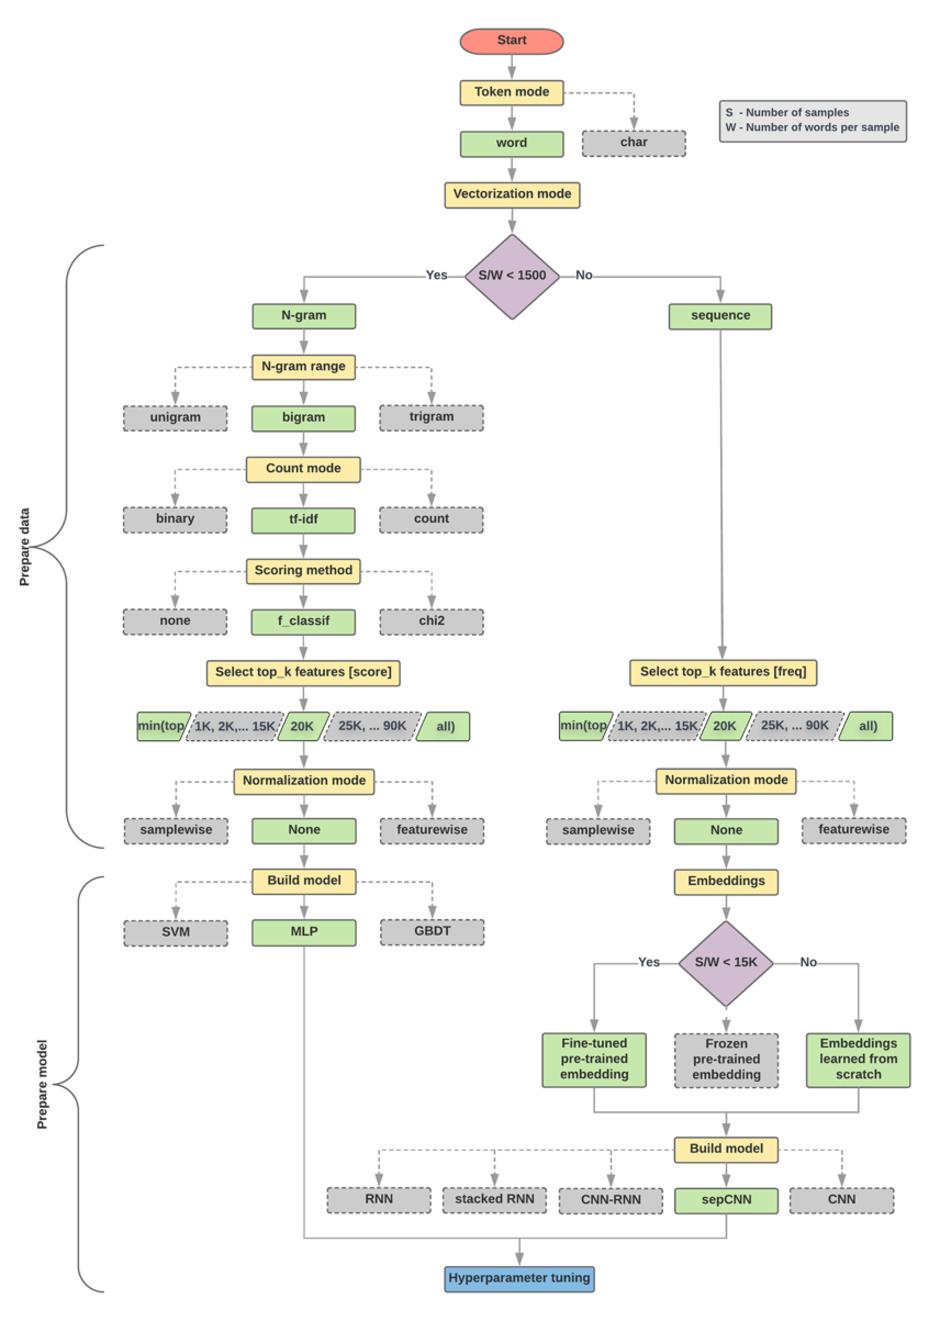
\includegraphics[width=\textwidth]{figures/chapter-5/GooglePlan.pdf}
    \caption[GooglePlan]{Text Classification Flowchart \parencite{google2021TCF}.
    \label{fig:GooglePlan}}
\end{figure}

\section{Supervision}

The development of the project model is based on a supervised approach due to the datasets located, it was most appropriate to use a supervised approach due to the datasets having no labels or lexical categories to train the model on; the model has user input to account for missing labels on data which have been manually and algorithmically added. The supervision for this project can be represented as the following diagram:

\begin{figure}[H]
    \centering
    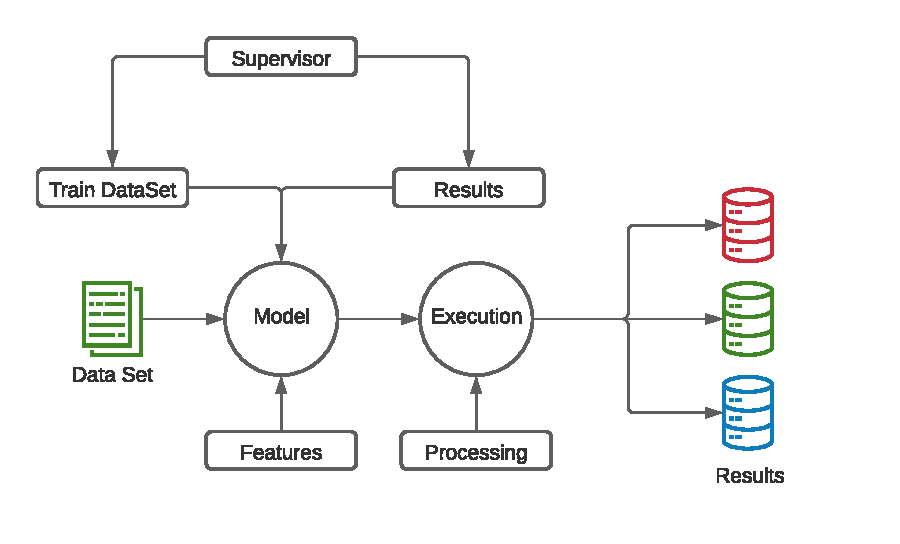
\includegraphics[width=\textwidth]{figures/chapter-5/SupervisedLearningChart.pdf}
    \caption[SupervisedLearning]{Sequence control for Supervised learning.
    \label{fig:SupervisedLearningChart}}
\end{figure}

\section{Pipeline Design}

\begin{figure}[H]
    \centering
    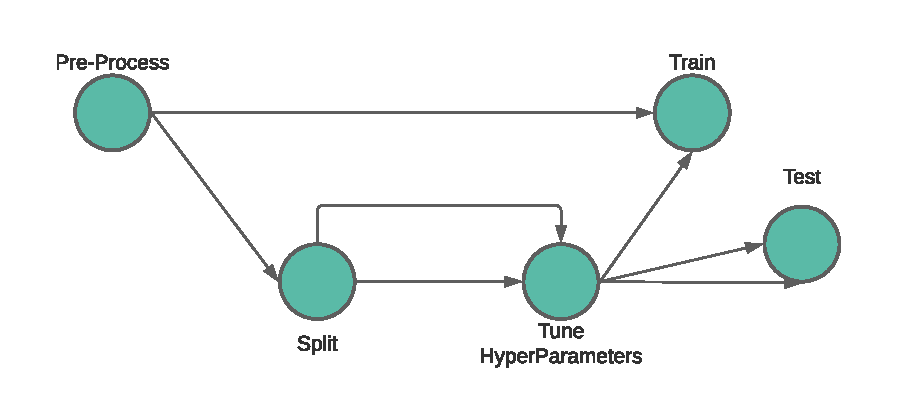
\includegraphics[width=\textwidth]{figures/chapter-5/Pipeline.pdf}
    \caption[MLTCPipeline]{Pipeline for model classification.
    \label{fig:MLTCPipeline}}
\end{figure}

There are five main steps for a text classification pipeline:

\begin{enumerate}
    \item \textbf{\textit{Pre-processing}}: prepare the raw dataset to be trained.
    \item \textbf{\textit{Splitting}}: split the processed dataset to be trained and validated.
    \item \textbf{\textit{Tuning}}: identity valuable parameters within trained data.
    \item \textbf{\textit{Training}}: train the current iteration of the model with updated hyper-parameters.
    \item \textbf{\textit{Testing}}: test and collect statistics for analysis to make further predictions.
\end{enumerate} \newpage

% FIXME
% \section{Data Preparation, Pre-processing, and Analytics}
\section[Data Preparation, Pre-processing, and Analytics]{\texorpdfstring{Data Preparation, Pre-processing, and \\ Analytics}{Data Preparation, Pre-processing, and Analytics}}

Preparing and pre-processing of the parsed data enables meaning to be allocated to the processed classification information, bypassing the implementation of a pre-processing step will ruin the chances of yielding valid returned data and will most likely detract meaning from any results throughout data analysis. The preparation and pre---preprocessing of data will be completed with the use of NLP libraries such as `pandas' and `sklearn'.

\subsection{Data Organisation and Binding}

The initial steps for data organisation will be to tidy the datasets procured from Kaggle as they held a lot of useless information and or columns with little weight. The first organisation step is to merge multiple CSV files and their respected columns into an easily readable format. The removal of unnecessary columns will aid the preprocessing as the dataset will be smaller.

\subsection{Pre-processing} \label{sub:C5Preprocessing}

The following methods of preprocessing will be applied to a given dataset:

\begin{itemize}
    \item \textbf{\textit{Punctuation:}} removal of all unnecessary punctuation, where punctuation includes the regular expression: \verb|["[.!?\\-]"]|.
    \item \textbf{\textit{Missing Values:}} word features with a percentage higher than the defined threshold for missing values will be sliced from the dataset as missing features will cause unreliable training data.
    \item \textbf{\textit{Collinear features:}} features in which are highly correlated with another lexical unit will be removed as these features can decrease overall performance on training data, this is due to higher variance of the similar features and lower interpretability of the model.
    \item \textbf{\textit{Stopwords:}} stopwords found within the given dataset will be removed as they do present meaning for classifcation as they are mostly common words such as "and" or "a", removing stopwords also has a positive affect on performance.
\end{itemize}
\chapter{Implementation}

implementation

\begin{python}
    def printIAmFukd(True):
        return False
\end{python}

\chapter{Evaluation and Testing}

Evaluation

\section{Aims and Objectives Evaluation}

Aims and Objectives

\begin{table}[H]
    \centering
    \begin{tabular}{lll}
    \hline
    \multicolumn{1}{|l|}{\textit{\textbf{Aim and Objective}}} & \multicolumn{1}{l|}{\textit{\textbf{Description}}} & \multicolumn{1}{l|}{\textit{\textbf{Satisfied - Yes/ No}}} \\ \hline
    21 & 22 & \multicolumn{1}{c|}{24} \\
    31 & 32 & \multicolumn{1}{c|}{34} \\
    41 & 42 & \multicolumn{1}{c|}{44} \\ \hline
    \end{tabular}
    \caption{Evaluation table for Aims and Objectives}
    \label{tab:EvaluationAimsAndObjectives}
\end{table}

\section{Methodology}

Methodology

\subsection{Project Plan}

Project Planning Evaluation

\section{Requirement Evaluation}

Requirement Evaluation

\subsection{Functional Evaluation}

\begin{table}[H]
    \centering
    \begin{tabular}{llll}
    \hline
    \multicolumn{1}{|l|}{\textit{\textbf{Requirement}}} & \multicolumn{1}{l|}{\textit{\textbf{Desired Outcome}}} & \multicolumn{1}{l|}{\textit{\textbf{Details}}} & \multicolumn{1}{l|}{\textit{\textbf{Satisfied - Yes/ No}}} \\ \hline
    21 & 22 & 23 & \multicolumn{1}{c|}{24} \\
    31 & 32 & 33 & \multicolumn{1}{c|}{34} \\
    41 & 42 & 43 & \multicolumn{1}{c|}{44} \\ \hline
    \end{tabular}
    \caption{Evaluation table for Functional Requirements}
    \label{tab:EvaluationFunctionalRequirements}
\end{table}

\subsection{Non-Functional Evaluation}

\begin{table}[H]
    \centering
    \begin{tabular}{llll}
    \hline
    \multicolumn{1}{|l|}{\textit{\textbf{Requirement}}} & \multicolumn{1}{l|}{\textit{\textbf{Desired Outcome}}} & \multicolumn{1}{l|}{\textit{\textbf{Details}}} & \multicolumn{1}{l|}{\textit{\textbf{Satisfied - Yes/ No}}} \\ \hline
    21 & 22 & 23 & \multicolumn{1}{c|}{24} \\
    31 & 32 & 33 & \multicolumn{1}{c|}{34} \\
    41 & 42 & 43 & \multicolumn{1}{c|}{44} \\ \hline
    \end{tabular}
    \caption{Evaluation table for Non-Functional Requirements}
    \label{tab:EvaluationNonFunctionalRequirements}
\end{table}

\section{Artefact Evaluation}

Artefact Evaluation

\subsection{Testing}



% Table templates for Chapter 7
% Table with 4 columns
% \begin{table}[]
%     \centering
%     \begin{tabular}{llll}
%     \hline
%     \multicolumn{1}{|l|}{\textit{\textbf{Title 1}}} & \multicolumn{1}{l|}{\textit{\textbf{Title 2}}} & \multicolumn{1}{l|}{\textit{\textbf{Title 3}}} & \multicolumn{1}{l|}{\textit{\textbf{Title 4}}} \\ \hline
%     21 & 22 & 23 & 24 \\
%     31 & 32 & 33 & 34 \\
%     41 & 42 & 43 & 44 \\ \hline
%     \end{tabular}
%     \caption{Table with 4}
%     \label{tab:TableWithFour}
% \end{table}

% % Table with 3 columns
% \begin{table}[]
%     \centering
%     \begin{tabular}{lll}
%     \hline
%     \multicolumn{1}{|l|}{\textit{\textbf{Title 1}}} & \multicolumn{1}{l|}{\textit{\textbf{Title 2}}} & \multicolumn{1}{l|}{\textit{\textbf{Title 3}}} \\ \hline
%     21 & 22 & 23 \\
%     31 & 32 & 33 \\
%     41 & 42 & 43 \\ \hline
%     \end{tabular}
%     \caption{Table with 3}
%     \label{tab:TableWith3}
% \end{table}
\chapter{Future Work}

This chapter focuses on possible amendments for this project, be it design or structural alterations for potential ideas to be constructed. The development carried out throughout this project has seen breakpoints which have led to new implementational ideas based on this project’s scope, entirely novel models which are a result of research (discussed in chapter 2). This chapter breaks down those ideas into their respected backgrounds and outlines future work and life for this project.

\section{Derived from Literature Review} \label{section:DerivedfromLiteratureReview}

As discussed in section \ref{section:IdentifyingResearchGapsandIncludingNovelty}, gaps can be identified within the research conducted, this section will focus on furthering the statements to explain how the literature review exposed less explored theoretical concepts and their counterpart implementation.

\begin{itemize}
    \item (Adaptation) --- \textbf{\textit{Compare POS-Tagging and Enhanced versions of Word2Vec with Machine Learning Implementations for Sentiment Analysis and Text Classification}}. Previous comparative studies focus on traditional versions of Word2Vec implementations, whereby it is often to see similar group-set of NLP and ML techniques being used in the results, this is a small change but could have a big impact for comparative studies and domain analysis. As ML concepts are now able to make use of more computational power, it is possible to phase out the testing of traditional techniques in favour for their ML adaptation (fundamentals do not change).
    \item (Novel Implementation) --- \textbf{\textit{Investigate the use of Machine Learning with Support-Vector Machines (SVM) and use Neural Networks or Deep Learning for Ensemble Learning applied Sentiment Analysis on Student Feedback.}}
\end{itemize}

\section{Derived from Artefact}

\subsection{Traditional Model}

N.Y.C

\subsection{Contemporary Model}

\subsubsection{Phrase Generation}

\begin{equation}
    \textbf{\textit{score}}(w_{a}, w_{b}) = \frac{\textbf{\textit{count}}(w_{a}w_{b}) - \delta}{\textbf{\textit{count}}(w_{a}) \times \textbf{\textit{count}}(w_{b})}
\end{equation}

\subsubsection{Subsampling}

\begin{equation}
    P(w_{i}) = 1 - \sqrt{\frac{t}{f(w_{i})}}
\end{equation}

\subsubsection{Negative Sampling}

\begin{equation}
    \log p(w | w_{i}) = \log \sigma ({v'}_{w}^{T} v_{w_{I}}) + \sum_{i=k}^{K} E_{w_{i}P_{n}(w)} \left [ \log \sigma (-{v'}_{w}^{T} v_{w_{I}}) \right ]
\end{equation}


\section{Derived from Observations}

When developing and training this project’s artefact, ethics were taken into consideration and it was decided to only make use of open-source (predefined) datasets, this decision limited the search for useable data and as a result, this model made use of two datasets from higher academic institutions. It would be beneficial to have access to more data or datasets for higher accuracy when training.

Expanding the model to an outside host, this project was developed within an isolated environment (the developer’s personal environment) as the model was easier to contain and maintain external variables. This resulted in limiting the nature of the model and its potential scope as resources were limited, however, developing in this state did minimise risk and lower the fault tolerance of the text-classification model. It would be beneficial to containerise this model and execute training on a more capable machine such as a higher core server.

The original intention for this project included the planning, design, and development of multiple NLP machine-learning models to put against each other to see how different implementations of theory may affect performance when trained on different datasets and NLP domains, however, due to unforeseen circumstances, this project experienced several difficulties with management and overall development. If this project were to have further development, it would be within reason to explore deeper theoretical combinations as discussed in section 8.1. The project’s scope and limitations would not differ as there is a pretrained and predefined model to use as a reference point.

\chapter{Conclusion}

% Recap what you did. In about one paragraph recap what your research question was and how you tackled it.
% Highlight the big accomplishments. Spend another paragraph explaining the highlights of your results. These are the main results you want the reader to remember after they put down the paper, so ignore any small details.
% Conclude. Finally, finish off with a sentence or two that wraps up your paper. I find this can often be the hardest part to write. You want the paper to feel finished after they read these. One way to do this, is to try and tie your research to the “real world.” Can you somehow relate how your research is important outside of academia? Or, if your results leave you with a big question, finish with that. Put it out there for the reader to think about to.
% Optional Before you conclude, if you don’t have a future work section, put in a paragraph detailing the questions you think arise from the work and where you think researchers need to be looking next.

Even though the mordern approach was not implemented, the mathematical foundations it is built on suggests it is a viable model as an alternative amalgamation with a potential accuracy of 96\% and a loss value of 40.65.


%%%%%%%%%%%%%%% APPENDICES
% \appendix

\begin{appendices}›
  \newpage

  \chapter{Project Initiation Document}
  
\includepdf[pages={1-8}]{PJE_UP853829_PID/PID_UP853829.pdf} \label{appendix:AppendixPID}

  \chapter{Ethics Review}
  % TODO update ethics form to have signature
  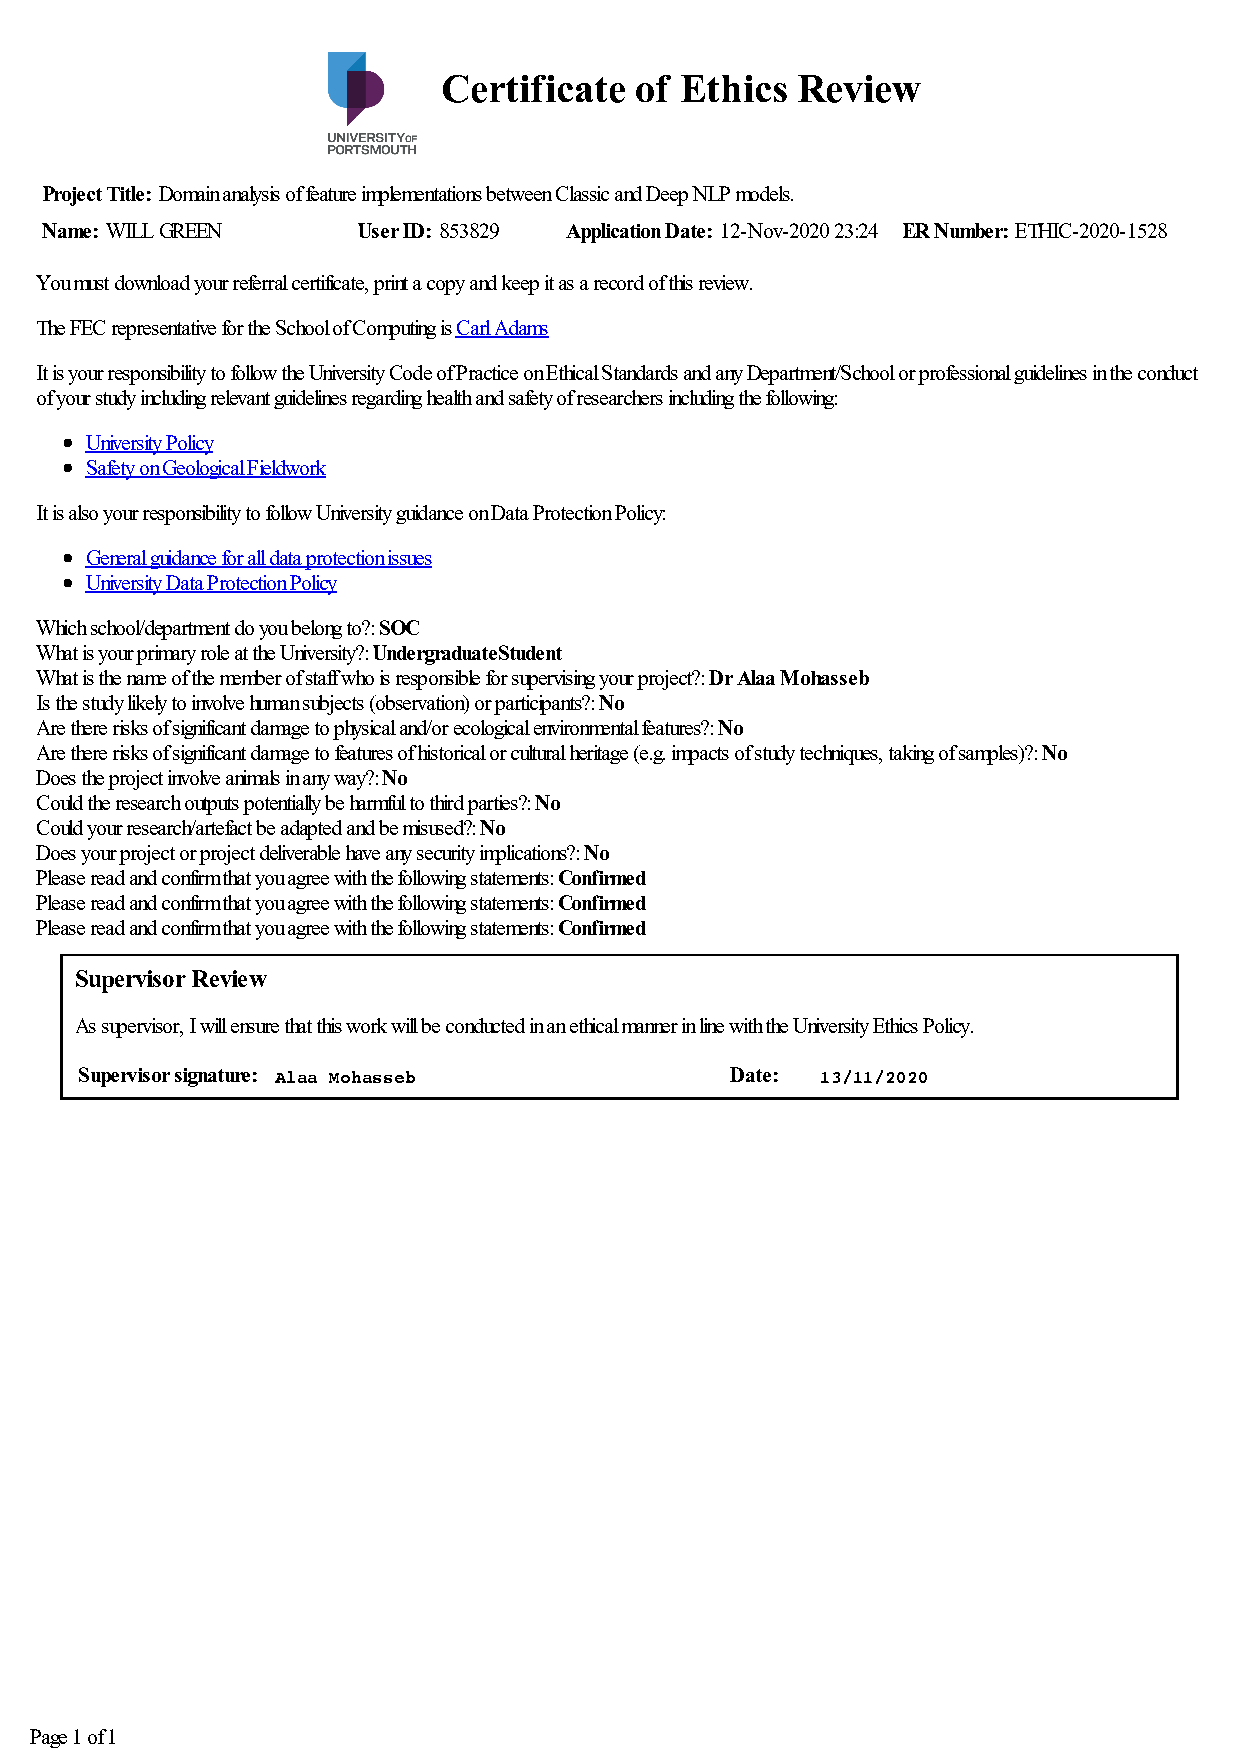
\includepdf[pages=-]{PJE_UP853829_PID/UP853829_Ethics_Form_Signed.png}
\end{appendices}

%%%%%%%%%%%%%% REFERENCES SECTION
\newpage
\phantomsection
\addcontentsline{toc}{chapter}{Bibliography}
% In order to try and get a consistent format I copy and paste the INSPIRE bibtex code into my bibtex file.
\printbibliography
\end{document}